% \iffalse meta-comment
%<*internal>
\iffalse
%</internal>
%<*readme>
----------------------------------------------------------------
phd-utils --- some useful uitlities
E-mail: yannislaz@gmail.com
Released under the LaTeX Project Public License v1.3c or later
See http://www.latex-project.org/lppl.txt
----------------------------------------------------------------
This file provides a phd for defining a class.
%</readme>
%<*readmemd>
###The `phd` LaTeX2e package

The `phd` latex package and the class with the same name provide
convenient methods to create new styles for books, reports
and articles. It also loads the most commonly used packages 
and resolves conflicts.

This work consists of the file  `phd.dtx`,
and the derived files   `phd.ins`,  `phd.pdf`, and `phd.sty`.

The `phd` bundle is a bunch of 15 packages, that manage all
aspects of document production.

They consist of:

1.0  The [phd-pkgmanager](https://github.com/yannisl/phd/blob/master/docs/phd-pkgmanager.md). This
     package manages all aspects of loading numerous packages and avoiding conflicts. It currently
     loads over 100 packages, directly or indirectly.
     
2.0  The [phd-fontmanager](https://github.com/yannisl/phd/blob/master/docs/phd-fontmanager.md). The
     `phd-fontmanager` sets up the fonts to be used for the document and provides an interface to
     all areas where font data is needed.
     
3.0  The [phd-handlers](https://github.com/yannisl/phd/blob/master/docs/phd-handlers.md). As we use
     extensively automatic key generation via code, this package provides numerous handlers.
     
4.0  The [phd-lowerlevelheadings](https://github.com/yannisl/phd/blob/master/docs/phd-lowerlevelheadings.md)     

5.0  The [phd-toc](https://github.com/yannisl/phd/blob/master/docs/phd-toc.md) package.
     Manages all aspects of Table of Contents via a key value interface. 

6.0  The [phd-counters](https://github.com/yannisl/phd/blob/master/docs/phd-counters.md) 

7.0  The [phd-colorpalette](https://github.com/yannisl/phd/blob/master/docs/phd-colorpalette.md). This
     package introduces the concept of a `color palette` to `LaTeX` coding. It groups all color
     data into `palettes`. By setting a single set of keys, the document can be updated with new
     color information.

8.0  The [phd-scriptsmanager](https://github.com/yannisl/phd/blob/master/docs/phd-scriptsmanager.md).
     Handles the settings and provides a key face interface to over scripts for use in typesetting
     texts from ancient to modern.

9.0  The [phd-documentation](https://github.com/yannisl/phd/blob/master/docs/phd-documentation.md).
     Provides numerous commands and keys for typesetting code. It also provides indexing shortcuts,
     including math symbols etc.
     
10.0 The [phd-epigraphs](https://github.com/yannisl/phd/blob/master/docs/phd-epigraphs.md).
     This package manages the typesetting of epigraphs.
     
11.0 The [phd-frontmatter](https://github.com/yannisl/phd/blob/master/docs/phd-epigraphs.md)
     package for the typesetting of frontmatter such as coverpages, copyright pages and title
     pages.
     
12.0 The [phd-lorems](https://github.com/yannisl/phd/blob/master/docs/phd-lorems.md)    
     package. Provides some additional commands for filler text.

13.0 The [phd-quote](https://github.com/yannisl/phd/blob/master/docs/phd-quote.md)    
     package. Provides some additional commands for filler text.
     
14.0 The [phd-lists](https://github.com/yannisl/phd/blob/master/docs/phd-lists.md)    
     package. Provides some additional commands and a key value interface for lists.  
     
15.0 The [phd-logos](https://github.com/yannisl/phd/blob/master/docs/phd-logos.md)    
     package. Supplementary commands for logos.         
      
###Installation

run
        `phd-lua phd.dtx` on windows
        
If you have any difficulties with the package come and join us at
http://tex.stackexchange.com and post a new question or
add a comment at http://tex.stackexchange.com/a/45023/963.
or send me a message at  yannislaz at gmail.com

### Documentation

The package was written using the `doc` and `docscript` packages,
so that it is self documented in a literary programming style. 
The .pdf is a fat document, providing over fifty book styles (the
equivalent of classes) plus there is a lot of write-up on the inner
workings of TeX and LaTeX2e. However, you don't need to know much
to use it.

      \usepackage{phd}
      \input{style13}

All choices, are made via an extended key-value interface. 
Although not a compliment, it resembles CSS and the keys are a bit verbose but
attributes are easy to change and have a consistent and easy to remember interface.

To set or add a key we only use one command:

      \cxset{chapter name font-size: Huge,
             chapter number font-size: HUGE} 

### Future Development

This is still an experimental version, but I will retain the
interface in future releases. There is a large amount of
work still to be carried out to improve the template styles
provided, to test it more thoroughly and to add a number of
improvements in the special designs. At present I estimate
that I have completed about 70% of the work that needs
to be done.

__The package as it stands is not production stable.__ 


%</readmemd>
%
%<*TODO>
1. On final round add pkg options. This was left as last in order not to solve problems by adding
    options. Too many options are not a good User Interface.
2.  Finish symbol management, both text and math. Math already 60% incorporated.
3.  Better integration of indexing commands.   
4.  Revisit layout manager for Chapters. Broke again in tests.
5.  Docs. Add all references.
6.  Incorporate phd class for more flexibility.
7. Improve package manager.
8. Group script loading for better font management.
9. General font management to relook it again.
10. Add all style sections (about 100 already prepared). Once they
     are all working issue beta version.
%</TODO>
%<*internal>
\fi
\def\nameofplainTeX{plain}
\ifx\fmtname\nameofplainTeX\else
  \expandafter\begingroup
\fi
%</internal>
%<*install>
\input l3docstrip.tex
\keepsilent
\askforoverwritefalse
\preamble
----------------------------------------------------------------
phd --- A package to beautify documents.
E-mail: yannislaz@gmail.com
Released under the LaTeX Project Public License v1.3c or later
See http://www.latex-project.org/lppl.txt
----------------------------------------------------------------
\endpreamble
%\BaseDirectory{C:/users/admin/my documents/github/phd}
%\usedir{MWE}
\generate{\file{\jobname.sty}{
  \from{\jobname.dtx}{package}
}}
%</install>
%<install>\endbatchfile
%<*internal>
%\usedir{tex/latex/phd}
\generate{
  \file{\jobname.ins}{\from{\jobname.dtx}{install}}
}
\nopreamble\nopostamble

\generate{
	\file{README.txt}{\from{\jobname.dtx}{readme}}
  }

\generate{
  \file{README.md}{\from{\jobname.dtx}{readmemd}}
}
\generate{
  \file{TODO.tex}{\from{\jobname.dtx}{TODO}}
}

\ifx\fmtname\nameofplainTeX
  \expandafter\endbatchfile
\else
  \expandafter\endgroup
\fi
 
\immediate\write18{makeindex -s gglo.ist -g phd.gls phd.glo}  %needs checking from trivfloat
\immediate\write18{makeindex -s gind.ist -g phd.ind phd.idx} %needs checking from Joseph’s trivfloat
%</internal>
%<*driver>
\NeedsTeXFormat{LaTeX2e}[2017/04/15]%
\documentclass[doctype=book,oneside,10pt,a4paper,colorize=true]{phddoc}
\usepackage{phdfilecontents}
\def\partname{Part}
\let\HUGE\huge
\usepackage[bottom=2cm]{geometry}
\savegeometry{std}
%\usepackage[microtype=on]{phd}
%\usepackage{phd-pkgmanager}
%\usepackage{phd-fontmanager}
\usepackage{phd-runningheads}
\usepackage{phd-lowersections}
\usepackage{phd-documentation}
\usepackage{phd-toc}
\sethyperref
\usepackage{makeidx}
\makeindex
\cxset{
%part format=stewart,
%       chapter afterindent=on,
       subsection afterindent=off,
%       part afterindent=on,
%       section format=hang,
%       chapter format=block,
%       chapter opening=left
}
       
\begin{document}
\DEBUGOFF

\frontmatter
\tableofcontents
%\listoffigures
%\listoftables
\mainmatter
\pagestyle{headings-sugar-hearts}
\parindent1em
\parindent1em
\chapter{The Basic LaTeX3 Syntax and Approach}
 \label{ch:l3intro}
 \cxset{epigraph width=0.7\textwidth}
 \epigraph{A final hint: listen carefully to what language users say they
want, until you have an understanding of what they really want. Then
find some way of achieving the latter at a small fraction of the cost
of the former. This is the test of success in language design, and
of progress in programming methodology. Perhaps these two are the same
subject anyway.}{C.A.R. Hoare, 1973}

		
\epigraph{Frank, in case you needed encouragement, please bear this in mind: I'm very much down at the blunt end of (La)TeX -- almost a total end-user. Following an earlier recommendation in this Q\&A, I visited the expl3 manual and was scared witless... Hope you can understand that---it's not a complaint, just an indication of the intellectual/experience distance from here to there.}{---Brent.Longborough Mar 2 '12 at 9:02 at \href{https://tex.stackexchange.com/questions/45838/what-can-i-do-to-help-the-latex3-project/46427\#46427}{SX.TX}}
 
Niklaus Wirth, the developer of the Pascal language long back in the 70’s wrote a paper titled \emph{On the Design of Programming Languages}. In his paper Wirth advocated that an important aspect of language design is \emph{simplicity}. He later on described the lessons learnt from his own works as:\footnote{\protect\url{http://chrisposkitt.com/tag/wirth/}}:

\begin{enumerate}
\item Writing a program is difficult.
\item Writing a correct program is even more so.
\item Writing a publishable program is exacting.
\item Programs are not written. They grow!
\item Controlling growth needs much discipline.
\item Reducing size and complexity is the triumph.
\item Programs must not be regarded as code for computers, but as literature for humans.
\end{enumerate}

The LaTeX3 syntax can only be described with some awe as `different’, although it retains some remnants of 
\tex’s syntax retaining the backslash, it is so different that many developers and package writers have resisted its adoption irrespective of the fact that it offers some solid code. 

Resistance to the language is understandable and noticed early by Computer Science pioneers. Hoare wrote:


\begin{quotation}
A necessary condition for the achievement of any of these objectives
is the utmost simplicity in the design of the language. Without simplicity,
even the language designer himself cannot evaluate the consequences of his
design decisions. Without simplicity, the compiler writer cannot achieve
even reliability, and certainly cannot construct compact, fast and
- efficient compilers. But the main beneficiary of simplicity is the user
of the language. In all spheres of human intellectual and practical
activity, from carpentry to golf, from sculpture to space travel, the
true craftsman is the one who thoroughly understands his tools. And this
applies to programmers too. A programmer who fully understands his
language can tackle more complex tasks, and complete them quicker and
more satisfactorily than if he did not. In fact, a programmer's need
for an understanding of his language is so great, that it is almost
impossible to persuade him to change to a new one. No matter what the
deficiencies of his current language, he has learned to live with them;
he has learned how to mitigate their effects by discipline and documentation,
and even to take advantage of them in ways which would be impossible
in a new and cleaner language which avoided the deficiency.

It therefore seems especially necessary in the design of a new
programming language, intended to attract programmers away from their
current high level language, to pursue the goal of simplicity to an
extreme, so that a programmer can readily learn and remember all its
features, can select the best facility for each of his purposes, can
fully understand the effects and consequences of each decision, and can
then concentrate the major part of his intellectual effort to understanding
his problem and his programs rather than his tool.
\end{quotation}

I have been programming for many years and have a disdain for languages that---as Hoare
put it--- I cannot remember ``all its features’’.  LaTeX3 has not achieved the level of simplicity required in its core. As a tool it fails the simplicity test and effortful learning is necessary to use it effectively. Currently there are probably less than twenty developers that understand it fully. 

Where, \latex3 excels is its architecture, overall plan and direction and modularizing the code to an extend that the required tools reside in logically set modules or classes in \latex’s terminology. What I can promise you, once you master it, there is no looking back. 

\section{Is it stable?}

One question that often arises is the stability of the current \latex~3 code base. Of course the degree to which software are “stable enough” depends on the requirements. Joseph Wright, answering a question on the SX.TX Q\&A site wrote:

\begin{latexquotation}
If you want 'will never change again', then plain TeX is probably your best bet. Knuth does still fix bugs periodically, but most things are now likely to be regarded as 'features' rather than bugs and so it's extremely likely that a document written in plain today will still work totally unchanged in tens of years (assuming TeX systems continue to be available).

The LaTeX2e kernel is also very unlikely to change further, and so is almost if not quite as stable as TeX itself. The team do fix bugs and do allow a bit more leeway than Knuth does, but even so it's extremely unlikely anything will change with LaTeX2e at the kernel level in a way that would require changes in documents.

There are some LaTeX packages one could reasonably decide to use which are also very stable and unlikely to see changes, either because they are no longer being actively developed or because the authors are careful to only change code related to genuine bugs or new, non-breaking, features. Obvious candidates are keyval, graphicx, etc.: probably there is actually quite a decent list, depending on your requirements.

In the case of the LaTeX3 packages l3kernel and l3packages, 'stable' does not extend as far as 'you will never have to make a change to a document using them', at least at this stage. What it means is that the team will not be making 'arbitrary' changes and will document/announce when this happens. Most of l3kernel is 'done', with the plans primarily focused on addition of new functionality rather than altering existing code. However there are a few places where we know some change may be required, and that will be announced on the LaTeX-L mailing list and documented. Even within these changes, 'breaking' (non-back-compatible) alterations will be small in number, but there is at least one of them we still need to do.

In the case of xparse, \docAuxCommand*{DeclareDocumentCommand} and so on are 'stable' in the sense that they will only be augmented, not removed, but there could be some changes on the more esoteric functions (for example, there are questions centred on the \textbf{g} argument type).

Thus 'stable enough' depends on your use case. If you can live with 'will have to make very occasional changes based on documented and scheduled updates' then expl3 is entirely usable. (I and others use if routinely in packages.) On the other hand, if you want 'this code must work with no changes with all future releases of support code' then we are not quite there yet.
\end{latexquotation}

\section{Getting started}

Other than the obvious of making sure you have the latest distribution from the LaTeX3 repository, 
the first step is to understand the conventions used by the \LaTeX3 developers. Macros are termed \meta{functions} and \meta{variables}. Macro names in general use the underscore and the colon in their names.
This is by design and to be honest is part of what many developers are unhappy about. It does cut down on the readability of the code and the longer names are more difficult to remember. This type of naming convention is similar to Hungarian notation, in which the name of a variable or function indicates its type  or its intended use and it does not have a lot of friends. Unlike \latex2e, expl3 uses the |:| and the underscore |_| extensively to produce |snake_case| like variables and functions. As such if the code is to be used together with \latex2e the code has to be run in a category regime in which spaces are ignored and the |_| and |:| are treated as \enquote{letters}. In this respect the functions |ExplSyntaxOn| and |ExplSyntaxOff| are provided. One of the advantages of |expl3| is that all spaces are ignored, avoiding a lot of issues with missing (\%) and unwanted spaces creeping into typeset material. 


Consider the \tex primitive \docAuxCommand*{meaning}. In \latex3 it has been remapped to \docAuxCommand*{token_to_meaning:N}. Similarly \docAuxCommand*{scan_stop:} has been let to \docAuxCommand*{relax}. We will define 

\begin{texexample}{Getting started}{ex:meaning}
\ExplSyntaxOn
% Define somevar in TeX style
\def\somevar{one}
% Get the meaing in TeX style
\meaning\somevar \\

% The LaTeX3 way
\token_to_meaning:N \somevar \\
\token_to_meaning:N \token_to_meaning:N
\token_to_meaning:N \scan_stop:  \\
\ExplSyntaxOff
\end{texexample}

So what is the advantage of the \latex3 conventions and usually longer names? Firstly as mentioned earlier, by using the convention we namespace our macros and this in itself can avoid errors. In a more canonical form we would write part of the earlier example as:

\begin{texexample}{Getting started}{ex:namespacing}
\ExplSyntaxOn
\cs_set:Npn \l_my_somevar:n #1 {#1}
\l_my_somevar:n {one}
\ExplSyntaxOff
\end{texexample}

As you will observe, we have some unfamiliar syntax but the underlying code is still the same. This time I have introduced |:n| at the tail of the function name.

The part that comes after the colon is termed the \emph{function signature}. For example in |token_to_meaning:N| in Example~\ref{ex:meaning}, the function signature is the \textbf{N}. The individual letter \enquote{N} is termed the argument specifier. Another important part is the prefix of the functions. There are some exceptions but the prefix normally indicates the module where the macro has been defined. So |\token_to_meaning:N|  can be found in the |l3token| package.\footnote{The term module and package are used interchangeably by the \latex3 Team.} The prefixes |l| or |g| are used to indicate local and global variables.
One is not forced to use the conventions for prefixes and |_|, however not using them defeats one of the main purposes of \latex3 which is to force developers to namespace their code.

There are a lot of advantages hiding behind the specifier part. By using the argument specifier, the new kernel
provides families of related functions which avoid the
need for complex |\expandafter| runs. For example,
the \tex primitive |\let| can only be used with a
macro name and a single token; no braces. In latex, the family of |\let|-like macros contains:\tcbdocmarginnote{U 2018-01-05}

\begin{texexample}{let with no expandafters}{ex:l3let}
\ExplSyntaxOn
\cs_set:Npn \Macro_Two {macro two replacement text}
\cs_set_eq:NN \Macro_One \Macro_Two
\cs_set_eq:Nc \Macro_One {Macro_Two}
\cs_set_eq:cN {Macro_One} \Macro_Two
\cs_set_eq:cc {Macro_One} {Macro_Two}

\cs_meaning:N \Macro_One

\ExplSyntaxOff
\end{texexample}

We can also write our own variants easily which we can explore a bit later.


Consider the definition of a simple function  |\phd_print_xy:nn| that accepts two values $x,y$ and prints them. This can be defined by one of the |cs_| type functions.

One way we could have defined the macro using  \tex would be:

\begin{teXXX}
\def\phdprint #1#2{x#1 y#2}
\end{teXXX}

Using \latexe we would have probably used |\newcommand| and if the definition was internal to a package used an |@|. 

\begin{teXXX}
\makeatletter
\newcommand\phd@print [2] {x#1 y#2}
\makeatother
\end{teXXX}

In \latex3 we would use |\cs_set_no_par:Npn|.

\begin{teXXX}
\cs_set_nopar:Npn \phd_print_xy:nn #1#2 { x #1 y #2 }
\end{teXXX}

So what is this mysterious |\cs_set_nopar:Npn|? We can find out by peeking at its meaning. This is shown in Example~\ref{ex:somemeaning}. As you can see behind the new dress is Knuth’s same old workhorse |\def|.

\begin{texexample}{The meaning of a command}{ex:somemeaning}
\ExplSyntaxOn
\token_to_meaning:N  \cs_set_nopar:Npn
\ExplSyntaxOff
\end{texexample}

But first let us examine the |:Npn| part of the |\cs_set_no_par:Npn| more carefully. What this means is the macro has three arguments. The first one is |N-type| which is a \tex token. The second one is |p-type|, which denotes normal \tex parameters such as |#1#2|. Lastly the |n-type| can be either a single token or a bracketted parameter. 

There are many more argument specifiers. Functions can be found with different argument specifiers and these are termed \emph{variants}. Recall that a macro can be defined using |\def|, |\edef| or a |\csname| construct. The argument specifier to the |\cs_setnopar| can be varied to achieve it. 

\begin{texexample}{The meaning of a command}{ex:somemeaning}
\ExplSyntaxOn
\token_to_meaning:N  \cs_set:Npn\\
\token_to_meaning:N  \cs_set_nopar:Npx\\
\token_to_meaning:N  \cs_set_nopar:cpx
\ExplSyntaxOff
\end{texexample}

Consider the use  of a |\csname| construct to define our |\phd_print_xy:nn| macro. The example that follows

\begin{texexample}{ex:csname}{ex:csname}

\ExplSyntaxOn
\expandafter\def\csname phd_print_xy:nn\endcsname #1 #2{x#1 y#2}

\token_to_meaning:N \phd_print_xy:nn\\

\cs_set_nopar:cpx {phd_print_xy:nn} #1 #2 {x#1 y#2}
\token_to_meaning:N \phd_print_xy:nn\\
\ExplSyntaxOff
\end{texexample} 

By using \latex3 functions, we do not need to use the |\expandafter| macro. The macro names are generally longer but the overall code is shorter.

So far we have used the |\token_to_meaning:N|. \latex3 offers similar commands to get the argument specification, the prefix and the replacement specification. When we specify a macro in \latex3 we can capture all its constituent parts and handle them individually if we want.

\begin{texexample}{Dissecting a macro}{ex:dissectmacro}
\ExplSyntaxOn

\cs_set_nopar:Npn \phd_print_xy:nn #1#2! { x #1 y #2 }
Macro meaning: \token_to_meaning:N \phd_print_xy:nn \\
Macro argument specification: \token_get_arg_spec:N \phd_print_xy:nn  \\
Prefix Spec: \token_get_prefix_spec:N \phd_print_xy:nn\\
Replacement Spec: \token_get_replacement_spec:N \phd_print_xy:nn

\ExplSyntaxOff
\end{texexample}


Some argue that the syntax is not syntactic sugar but syntactic cyanide that changes the look and feel both of \latexe and \tex command macros. You should think of |expl3| as a new computer language. It does introduce consistency and offers a full repertoire of tools. The syntactic strangeness of the language does introduce barriers to mastering it, but the advantages far outweigh the difficulties of the language.


The eye tends to miss the argument specifier, it is important to note that the macro
name is \cmd{\test\_something:nn} and not \cmd{\test\_something} and the factory command is |\cs_new:Npn| and not |\cs_new|. If you have been programming using traditional macros this is a common mistake that you will accidentally make and you will get an |error unknown| message.


\section{Where from here}

The chapters of this book follow a logical sequence for learning the language, although most of them can be read as stand alone. 

The steps in learning any computer language require a logical sequence of study:

\begin{enumerate}
\item Understanding the syntax
\item Variables and datatypes
\item Numbers and assignments
\item Control Structures
\item Functions
\item Data structures
\item Ecosystem
\end{enumerate}

In the next chapter we would study the creation of functions in more detail. This is the most important skill to master before you proceed with the rest of the programming constructs, such as iteration, arithmetic operations etc.



\chapter{Defining Functions and Variables}

\section{Defining functions}
There are two main methods to define functions. In the first method you are required to use parameter tex, whereas in the second this can be left out, as it can be inferred from the argument specification of the function being defined. The functions used to create other functions can be found in both forms. For example:

\begin{texexample}{Using parameter text}{}
\ExplSyntaxOn
\cs_set_nopar:Npn \phd_print:n #1 {#1}
\token_to_meaning:N \phd_print:n\\

\cs_set_nopar:Nn  \phd_print:n  {#1}


\cs_meaning:N \phd_print:n\\
\ExplSyntaxOff
\end{texexample}



 Functions can be created with no requirement that they are declared
 first (in contrast to variables, which must always be declared).\footnote{This primarily refers to variables that require a \tex register.}
 Declaring a function before setting up the code means that the name
 chosen will be checked and an error raised if it is already in use.
 The name of a function can be checked at the point of definition using
 the \docAuxCommand*{cs_new}\ldots functions: this is recommended for all
 functions which are defined for the first time.

 There are three primary ways to define new functions, using |new|, |set| or |gset| variations.  The first one is similar to the \latexe |\newcommand|, and produces macros that will generate an error if there is an attempt to redefine them. The other two are variations of the |\def or \edef| and |\gdef or \xdef| \tex commands.
 
 All classes define a function to expand to the substitution text.
 Within the substitution text the actual parameters are substituted
 for the formal parameters (|#1|, |#2|, \ldots).
 
 \begin{description}
   \item[\texttt{new}]
     Create a new function with the \texttt{new} scope,
     such as \docAuxCommand* {cs_new:Npn}.  The definition is global and will result in
     an error if it is already defined.
   \item[\texttt{set}]
     Create a new function with the \texttt{set} scope,
     such as \docAuxCommand* {cs_set:Npn}. The definition is restricted to the current
     \TeX{} group and will not result in an error if the function is already
     defined.
   \item[\texttt{gset}]
     Create a new function with the \texttt{gset} scope,
     such as \docAuxCommand* {cs_gset:Npn}. The definition is global and
     will not result in an error if the function is already defined.
 \end{description}

  Finally, the functions in
 Subsections~\ref{sec:l3basics:defining-new-function-1}~and
 \ref{sec:l3basics:defining-new-function-2} are primarily meant to define
 \emph{base functions} only. Base functions can only have the following
 argument specifiers:
 \begin{description}
   \item[|N| and |n|] No manipulation.
   \item[|T| and |F|] Functionally equivalent to |n| (you are actually
     encouraged to use the family of |\prg_new_conditional:| functions
     described in Section~\ref{sec:l3prg:new-conditional-functions}).
   \item[|p| and |w|] These are special cases.
 \end{description}



 Within each set of scope there are different ways to define a function.
 The differences depend on restrictions on the actual parameters and
 the expandability of the resulting function.
 \begin{description}
   \item[\texttt{nopar}]
      Create a new function with the \texttt{nopar} restriction,
      such as \docAuxCommand*{cs_set_nopar:Npn}. The parameter may not contain
      \docAuxCommand*{par} tokens.
   \item[\texttt{protected}]
      Create a new function with the \texttt{protected} restriction,
      such as \docAuxCommand*{cs_set_protected:Npn}. The parameter may contain
      \docAuxCommand*{par} tokens but the function will not expand within an
      \texttt{x}-type expansion.
 \end{description}
 
 
\subsection{Defining new functions using parameter text}

Theses function are \TeX ish in style, as compared to those functions that use the signature to automatically detect the number of parameters and are more \LaTeX-like. They are mainly used with the |:Npn| signature specification.

\begin{texexample}{Using parameter text}{}
\ExplSyntaxOn
\cs_new:Npn \phd_print:n #1 {#1}

\token_to_meaning:N \cs_new:Npn\\
\token_to_meaning:N \phd_print:n
\ExplSyntaxOff
\end{texexample}

\begin{docCommand}{cs_new:Npn} {\meta{function} \meta{parameters} \marg{code}}
Creates \meta{function} to expand to \meta{code} as replacement text. Within the \meta{code}, the
\meta{parameters} (\#1, \#2, etc.) will be replaced by those absorbed by the function. The
definition is \textbf{global} and an error will result if the \meta{function} is already defined.
Variants with |cpn,Npx,cpx| are predefined by the kernel.
\end{docCommand}

The |:Npn| form can also be used even if there is no parameter text. However this is considered a constant variable and is preferred to be coded as a |tl| such.

\begin{texexample}{Usage of the macro}{ex:csnew}
\ExplSyntaxOn
  \cs_new:Npn \copyrightfootnote: 
    {
      \footnotetext{Copyright~(2014-2015)~of~Yiannis~Lazarides,~distributed~
      under~the~\LaTeX{}~Project~Public~License~(LPPL).}
    }
  \copyrightfootnote:
\ExplSyntaxOff
\end{texexample}

An important point to note is if you use the function signature type you will get an error if the trailing |:| is not used in the macro name. 

\begin{teXXX}
\cs_new:Nn \copyrightafootnote 
  {
    ...
  }
\copyrightafootnote
\end{teXXX}

This will produce an error:\ExplSyntaxOn\copyrightfootnote:\ExplSyntaxOff

\begin{verbatim}
! LaTeX error: "kernel/missing-colon"
! Function '\copyrightafootnote' contains no ':'.
! See the LaTeX3 documentation for further information.
! For immediate help type H <return>.
\end{verbatim}

If the function is redefined, it will produce an error, similar to \latexe |\newcommand|. However, do note that the |set| family of commands can silently overwrite it. 

\begin{texexample}{Usage of the macro \protect\string\cs\_gset:Npn}{ex:csnew}
\ExplSyntaxOn
\cs_gset:Npn \copyrightfootnote: {\footnotetext{Copyright~(2014-2015)~of~
         Yiannis~Lazarides,~distributed~
         under~the~\LaTeX{}~Project~Public~License~(LPPL).}}
\copyrightfootnote:
\ExplSyntaxOff
\end{texexample}

\begin{docCommand}{cs_new_nopar:Npn} {\meta{function} \meta{parameters} \marg{code}}
Creates \meta{function} to expand to \meta{code} as replacement text. Within the \meta{code}, the
\meta{parameters} (\#1, \#2, etc.) will be replaced by those absorbed by the function. When the
\meta{function} is used the hparametersi absorbed cannot contain \par tokens. The definition
is global and an error will result if the \meta{function} is already defined.
\end{docCommand}

\begin{texexample}{Meaning}{}
\ExplSyntaxOn
\token_to_meaning:N \cs_new_nopar:Npn
\ExplSyntaxOff
\end{texexample}

\begin{docCommand}{cs_new_protected:Npn}{\meta{function} \meta{parameters} \marg{code}}
Creates \meta{function} to expand to \meta{code} as replacement text. Within the hcodei, the
hparametersi (\#1, \#2, etc.) will be replaced by those absorbed by the function. The
\meta{function} will not expand within an x-type argument. The definition is global and an
error will result if the hfunctioni is already defined.
\end{docCommand}

\begin{docCommand}{cs_new_protected_nopar:Npn}{\meta{function} \meta{parameters} \marg{code}}
Creates \meta{function} to expand to \meta{code} as replacement text. 
When the \meta{function} is used the \meta{parameters} absorbed cannot contain \docAuxCommand*{par} tokens. The hfunctioni
will not expand within an x-type argument. The definition is global and an error will
result if the \meta{function} is already defined.
\end{docCommand}

This brings us to the end of the |new| type functions that can be used for function definitions. They all have variants of the form |cpn| and |cpx| and the base function for edef also is available. You can consult the manual for more definitions.

\subsubsection{The set type functions}

The rest of the commands are variations using the \cs{cs_}\meta{set} form of function creating macros. These do not issue a  warning if redefined.

 \begin{docCommand}{cs_set:Npn} {\meta{function} \meta{parameters} \marg{code}}
   Sets \meta{function} to expand to \meta{code} as replacement text.
   Within the \meta{code}, the \meta{parameters} (|#1|, |#2|,
   \emph{etc.}) will be replaced by those absorbed by the function.
   The assignment of a meaning to the \meta{function} is restricted to
   the current \TeX{} group level.
\end{docCommand}

\begin{texexample}{Meaning}{}
\ExplSyntaxOn
\token_to_meaning:N \cs_set:Npn
\ExplSyntaxOff
\end{texexample}

As can be seen from the example this is |\protected \long \def|. The |\cs_set_nopar:Npn| in the maeaning in the example is described next and is simply an equivalent function to |\def|.

 \begin{docCommand} {cs_set_nopar:Npn}{\meta{function} \meta{parameters} \marg{code}}
   Sets \meta{function} to expand to \meta{code} as replacement text.
   Within the \meta{code}, the \meta{parameters} (|#1|, |#2|,
   \emph{etc.}) will be replaced by those absorbed by the function.
   When the \meta{function} is used the \meta{parameters} absorbed
   cannot contain \cs{par} tokens. The assignment of a meaning
   to the \meta{function} is restricted to the current \TeX{} group
   level.
 \end{docCommand}
 
 \begin{texexample}{Meaning \textbackslash cs\_set\_nopar:Npn}{}
\ExplSyntaxOn
\token_to_meaning:N \cs_set_nopar:Npn
\ExplSyntaxOff
\end{texexample}
 

\begin{docCommand}{cs_set_protected:Npn} {\meta{function} \meta{parameters} \marg{code}}
   Sets \meta{function} to expand to \meta{code} as replacement text.
   Within the \meta{code}, the \meta{parameters} (|#1|, |#2|,
   \emph{etc.}) will be replaced by those absorbed by the function.
   The assignment of a meaning to the \meta{function} is restricted to
   the current \TeX{} group level. The \meta{function} will
   not expand within an \texttt{x}-type argument.
 \end{docCommand}
 \begin{texexample}{Meaning \textbackslash cs\_set\_protected:Npn}{}
 \ExplSyntaxOn
 \token_to_meaning:N \cs_set_protected:Npn
\ExplSyntaxOff
\end{texexample}
 


\begin{docCommand}{cs_set_protected_nopar:Npn}{\meta{function} \meta{parameters} \marg{code}}
   Sets \meta{function} to expand to \meta{code} as replacement text.
   Within the \meta{code}, the \meta{parameters} (|#1|, |#2|,
   \emph{etc.}) will be replaced by those absorbed by the function.
   When the \meta{function} is used the \meta{parameters} absorbed
   cannot contain \cs{par} tokens. The assignment of a meaning
   to the \meta{function} is restricted to the current \TeX{} group
   level. The \meta{function} will not expand within an
   \texttt{x}-type argument.
\end{docCommand}
\begin{texexample}{Meaning \textbackslash cs\_set\_protected\_nopar:Npn}{}
\ExplSyntaxOn
\token_to_meaning:N \cs_set_protected_nopar:Npn
\ExplSyntaxOff
\end{texexample}
 
Next the above are made available by the \latex3 kernel but all in the |global| form of the command. The syntax is identical except they use |cs_gset|.


\begin{docCommand} {cs_gset:Npn}{\meta{function} \meta{parameters} \marg{code}}
   Globally sets \meta{function} to expand to \meta{code} as replacement
   text. Within the \meta{code}, the \meta{parameters} (|#1|, |#2|,
  \emph{etc.}) will be replaced by those absorbed by the function.
  The assignment of a meaning to the \meta{function} is \emph{not}
   restricted to the current \TeX{} group level: the assignment is
   global.
\end{docCommand}
\begin{texexample}{Meaning \textbackslash cs\_gset:Npn}{}
\ExplSyntaxOn
\token_to_meaning:N \cs_gset:Npn
\ExplSyntaxOff
\end{texexample}

\begin{docCommand}{cs_gset_nopar:Npn} {\meta{function} \meta{parameters} \marg{code}}
   Globally sets \meta{function} to expand to \meta{code} as replacement
   text. Within the \meta{code}, the \meta{parameters} (|#1|, |#2|,
   \emph{etc.}) will be replaced by those absorbed by the function.
   When the \meta{function} is used the \meta{parameters} absorbed
   cannot contain \cs{par} tokens. The assignment of a meaning to the
   \meta{function} is \emph{not} restricted to the current \TeX{}
   group level: the assignment is global.
\end{docCommand}
\begin{texexample}{Meaning \textbackslash cs\_gset\_nopar:Npn}{}
\ExplSyntaxOn
\token_to_meaning:N \cs_gset_nopar:Npn
\ExplSyntaxOff
\end{texexample}


\begin{docCommand} {cs_gset_protected:Npn} {\meta{function} \meta{parameters} \marg{code}}
   Globally sets \meta{function} to expand to \meta{code} as replacement
   text. Within the \meta{code}, the \meta{parameters} (|#1|, |#2|,
   \emph{etc.}) will be replaced by those absorbed by the function.
   The assignment of a meaning to the \meta{function} is \emph{not}
   restricted to the current \TeX{} group level: the assignment is
   global. The \meta{function} will not expand within an
   \texttt{x}-type argument.
\end{docCommand}
\begin{texexample}{Meaning \textbackslash cs\_gset\_protected:Npn}{}
\ExplSyntaxOn
\token_to_meaning:N \cs_gset_protected:Npn
\ExplSyntaxOff
\end{texexample}

\begin{docCommand}{cs_gset_protected_nopar:Npn} {\meta{function} \meta{parameters} \marg{code}}
   Globally sets \meta{function} to expand to \meta{code} as replacement
   text. Within the \meta{code}, the \meta{parameters} (|#1|, |#2|,
   \emph{etc.}) will be replaced by those absorbed by the function.
   When the \meta{function} is used the \meta{parameters} absorbed
   cannot contain \cs{par} tokens. The assignment of a meaning to the
   \meta{function} is \emph{not} restricted to the current \TeX{}
   group level: the assignment is global. The \meta{function} will
   not expand within an \texttt{x}-type argument.
\end{docCommand}
\begin{texexample}{Meaning \textbackslash cs\_gset\_protected\_nopar:Npn}{}
\ExplSyntaxOn
\token_to_meaning:N \cs_gset_protected_nopar:Npn
\ExplSyntaxOff
\end{texexample}

This brings us to the end of the functions available to the developer for defining macros. It’s a lot of them. In the next section some more functions are defined, this time using the signature of the function the function are created automatically without the need to type in the parameter text.


\subsection{Defining new functions using the signature}

The functions outlined below have a simpler form in that they create other commands without the need to specify their arguments. The number of parameters is detected automatically from the function signature. Which method is the best is obvious up to the user preferences.\footnote{See discussion at SX.TX \protect{\url{http://tex.stackexchange.com/questions/240675/differences-in-latex3-function-generation-methods}}} 


\begin{docCommand}{cs_new:Nn}{\meta{function}\marg{code}}
Creates \meta{function} to expand to \meta{code} as replacement text. A nice feature is that within the \meta{code}
the number of parameters is detected automatically from the function signature. These \meta{parameters} (\#1, \#2, etc.) will be replaced by those absorbed by the function. The definition is global and an error will result if the \meta{function} is already defined.\footnote{The definitions of the commands have been taken mostly verbatim from the documentation of the package.}


\begin{texexample}{Signature}{ex:signature}
\ExplSyntaxOn
\cs_new:Nn \exampleone:nn {}
\cs_new:Nn \exampletwo:nn{#1 #2}
\exampleone:nn {one}{two}

\exampletwo:nn{one }{two}

\texttt\textbackslash\cs_to_str:N\exampleone:nn
\ExplSyntaxOff
\end{texexample}
\end{docCommand}

 
 
 
\begin{docCommand}{cs_new_nopar:Nn}{\meta{function} \marg{code}}
   Creates \meta{function} to expand to \meta{code} as replacement text.
   Within the \meta{code}, the number of \meta{parameters} is detected
   automatically from the function signature. These \meta{parameters}
   (|#1|, |#2|, \emph{etc.}) will be replaced by those absorbed by the
   function.  When the \meta{function} is used the \meta{parameters}
   absorbed cannot contain \docAuxCommand*{par} tokens. The definition is global and
   an error will result if the \meta{function} is already defined.
 \end{docCommand}

\begin{function}[pTF]{\cs_if_exist:N}
\begin{docCommand}{cs_new_protected:Nn}{\meta{function} \marg{code}}
   Creates \meta{function} to expand to \meta{code} as replacement text.
   Within the \meta{code}, the number of \meta{parameters} is detected
   automatically from the function signature. These \meta{parameters}
   (|#1|, |#2|, \emph{etc.}) will be replaced by those absorbed by the
   function. The \meta{function} will not expand within an \texttt{x}-type
   argument. The definition is global and
   an error will result if the \meta{function} is already defined.
\end{docCommand}
\end{function}  

%
% \begin{function}
%   {
%     \docAuxCommand*_new_protected_nopar:Nn, \docAuxCommand*_new_protected_nopar:cn,
%     \docAuxCommand*_new_protected_nopar:Nx, \docAuxCommand*_new_protected_nopar:cx
%   }
%   \begin{syntax}
%     \docAuxCommand*{cs_new_protected_nopar:Nn} \meta{function} \Arg{code}
%   \end{syntax}
%   Creates \meta{function} to expand to \meta{code} as replacement text.
%   Within the \meta{code}, the number of \meta{parameters} is detected
%   automatically from the function signature. These \meta{parameters}
%   (|#1|, |#2|, \emph{etc.}) will be replaced by those absorbed by the
%   function.  When the \meta{function} is used the \meta{parameters}
%   absorbed cannot contain \docAuxCommand*{par} tokens. The \meta{function} will not
%   expand within an \texttt{x}-type argument. The definition is global and
%   an error will result if the \meta{function} is already defined.
% \end{function}

Similarly to the |cs_new| commands the |cs_set| functions create other commands, this time
with a local scope. This pattern is followed right through the kernel.

 \begin{docCommand}{cs_set:Nn}{\meta{function}\marg{code}}
   Sets \meta{function} to expand to \meta{code} as replacement text.
   Within the \meta{code}, the number of \meta{parameters} is detected
   automatically from the function signature. These \meta{parameters}
   (|#1|, |#2|, \emph{etc.}) will be replaced by those absorbed by the
   function.
   The assignment of a meaning to the \meta{function} is restricted to
   the current \TeX{} group level.
 \end{docCommand}

\begin{docCommand}{cs_set_nopar:Nn}{\meta{function}\marg{code}}
   Sets \meta{function} to expand to \meta{code} as replacement text.
   Within the \meta{code}, the number of \meta{parameters} is detected
   automatically from the function signature. These \meta{parameters}
   (|#1|, |#2|, \emph{etc.}) will be replaced by those absorbed by the
   function.  When the \meta{function} is used the \meta{parameters}
   absorbed cannot contain \docAuxCommand*{par} tokens.
   The assignment of a meaning to the \meta{function} is restricted to
   the current \TeX{} group level. This is the \tex primitive \docAuxCommand*{def}
\end{docCommand}

\begin{teX}
\tex_let:D \cs_set_nopar:Npn \tex_def:D
748 \tex_let:D \cs_set_nopar:Npx \tex_edef:D
749 \etex_protected:D \cs_set_nopar:Npn \cs_set:Npn
750                     { \tex_long:D \cs_set_nopar:Npn }
751 \etex_protected:D \cs_set_nopar:Npn \cs_set:Npx
752                   { \tex_long:D \cs_set_nopar:Npx }
753 \etex_protected:D \cs_set_nopar:Npn \cs_set_protected_nopar:Npn
754 { \etex_protected:D \cs_set_nopar:Npn }
755 \etex_protected:D \cs_set_nopar:Npn \cs_set_protected_nopar:Npx
756 { \etex_protected:D \cs_set_nopar:Npx }
757 \cs_set_protected_nopar:Npn \cs_set_protected:Npn
758 { \etex_protected:D \tex_long:D \cs_set_nopar:Npn }
759 \cs_set_protected_nopar:Npn \cs_set_protected:Npx
760 { \etex_protected:D \tex_long:D \cs_set_nopar:Npx }
\end{teX}
\ExplSyntaxOn
\meaning\cs_new:Npn
\ExplSyntaxOff


\begin{docCommand}{cs_set_protected:Nn}{\meta{function}\marg{code}}
   Sets \meta{function} to expand to \meta{code} as replacement text.
   Within the \meta{code}, the number of \meta{parameters} is detected
   automatically from the function signature. These \meta{parameters}
   (|#1|, |#2|, \emph{etc.}) will be replaced by those absorbed by the
   function. The \meta{function} will not expand within an \texttt{x}-type
   argument.
   The assignment of a meaning to the \meta{function} is restricted to
   the current \TeX{} group level.
 \end{docCommand}

\begin{docCommand}{cs_set_protected_nopar:Nn}{ \meta{function} \marg{code}}
   Sets \meta{function} to expand to \meta{code} as replacement text.
   Within the \meta{code}, the number of \meta{parameters} is detected
   automatically from the function signature. These \meta{parameters}
   (|#1|, |#2|, \emph{etc.}) will be replaced by those absorbed by the
   function.  When the \meta{function} is used the \meta{parameters}
   absorbed cannot contain \docAuxCommand*{par} tokens. The \meta{function} will not
   expand within an \texttt{x}-type argument.
   The assignment of a meaning to the \meta{function} is restricted to
   the current \TeX{} group level.
 \end{docCommand}

The next commands create functions with global scope.

 \begin{docCommand}{cs_gset:Nn}{ \meta{function} \marg{code}}
   Sets \meta{function} to expand to \meta{code} as replacement text.
   Within the \meta{code}, the number of \meta{parameters} is detected
   automatically from the function signature. These \meta{parameters}
   (|#1|, |#2|, \emph{etc.}) will be replaced by those absorbed by the
   function.
   The assignment of a meaning to the \meta{function} is  global.
 \end{docCommand}

 \begin{docCommand}{cs_gset_nopar:Nn}{ \meta{function} \marg{code}}
   Sets \meta{function} to expand to \meta{code} as replacement text.
   Within the \meta{code}, the number of \meta{parameters} is detected
   automatically from the function signature. These \meta{parameters}
   (|#1|, |#2|, \emph{etc.}) will be replaced by those absorbed by the
   function.  When the \meta{function} is used the \meta{parameters}
   absorbed cannot contain \docAuxCommand*{par} tokens.
   The assignment of a meaning to the \meta{function} is global.
 \end{docCommand}
 

\section{Copying control sequences}

Control sequences (not just functions as defined above) can be set to have the same
meaning using the functions described here. Making two control sequences equivalent
means that the second control sequence is a copy of the first (rather than a pointer to
it). Thus the old and new control sequence are not tied together: changes to one are not
reflected in the other. These are syntactic replacements for the \tex primitive|\let|.

\begin{texexample}{Let}{}
\ExplSyntaxOn
\cs_set_nopar:Nn \testa: {AAA}
\cs_set_eq:NN\testb: \testa:
\token_to_meaning:N \testa:  \\
\cs_set_nopar:Nn \testa: {BBBB}
\testb:  \\
\token_to_meaning:N \testb:  \\
\token_to_meaning:N \testa:  \\
\testa:\\
\testb: \\
\meaning\cs_set_eq:NN

% check if equal to \let
\token_to_meaning:N \let\\
\token_to_meaning:N \cs_set_equal:NN
\ExplSyntaxOff
\end{texexample}

 In the following text \enquote{cs} is used as an abbreviation for
 \enquote{control sequence}.

 \begin{docCommand}{cs_new_eq:NN} {\meta{cs1} \meta{cs2}}
   Globally creates \meta{control sequence 1} and sets it to have the same
   meaning as \meta{control sequence 2} or |<token>|.
   The second control sequence may
   subsequently be altered without affecting the copy.
\end{docCommand}


\begin{docCommand}{cs_set_eq:NN} {\meta{cs1} \meta{cs2}}
   Sets \meta{control sequence1} to have the same meaning as
   \meta{control sequence2} (or |<token>|).
   The second control sequence may subsequently be
   altered without affecting the copy. The assignment of a meaning
   to the \meta{control sequence1} is restricted to the current
   \TeX{} group level.
 \end{docCommand}


\begin{docCommand} {cs_gset_eq:NN} {\meta{cs1} \meta{cs2}}
   Globally sets \meta{control sequence1} to have the same meaning as
   \meta{control sequence2} (or |<token>|).
   The second control sequence may subsequently be
   altered without affecting the copy. The assignment of a meaning to
   the \meta{control sequence1} is \emph{not} restricted to the current
   \TeX{} group level: the assignment is global.
\end{docCommand}

\section{Undefining control sequences}

There are occasions where control sequences need to be deleted. This is handled in a
very simple manner by the use of 
|\cs_undefine:N| \meta{control sequence},
which sets \meta{control sequence} to be globally |undefined|.

\begin{texexample}{Undefining control sequences}{ex:undefine}
\ExplSyntaxOn
\cs_set_nopar:Npn \testa: {AAA}
\cs_set_nopar:cpn {testb} {AAA}

\cs_undefine:N \testa:
\cs_undefine:c {testb}
\token_to_meaning:N \cs_undefine:N\\

\token_to_meaning:N \testa:\\
\token_to_meaning:c {testb}\\
\token_to_meaning:N \token_to_meaning:c
\ExplSyntaxOff
\end{texexample}

The function would simply set the command to the \tex primitive |undefine|, as can be seen from the example.
There is another group of commands associated with constructor functions.

\section{Converting to and from control sequences}

\begin{docCommand}{cs_if_exist_use:N} {\meta{control sequence}}
Tests whether the \meta{control sequence} is currently defined (whether as a function or another
control sequence type), and if it does inserts the \meta{control sequence} into the input stream.
\end{docCommand}

\begin{docCommand}{cs_if_exist_use:NTF} {\meta{control sequence}}
Tests whether the \meta{control sequence} is currently defined (whether as a function or another
control sequence type), and if it does inserts the \meta{control sequence} into the input stream
followed by the \meta{true code}.
\end{docCommand}

\begin{texexample}{Converting to and from control sequences}{ex:ifexists}
\ExplSyntaxOn
\cs_if_exist_use:NTF \test {}{\FALSE}
\ExplSyntaxOff
\end{texexample}

Note that numerous times, I have typed |\cs_if_exists_use:NTF| rather than the more grammatical  |\cs_if_exist_use:NTF| with consequent errors. Grammar is hardwired in the brain and it requires mental effort to write ungrammatical commands. This is an issue that needs to be addressed by the \latex3 developers. 

The famous |\csname| is mapped in this section of the module as well. Unpredictably, it got a shorter name, but a weird suffix |w|! It deserves both as it is the workhorse of \tex. The remapped commands are formally described in the manual as shown below:

\begin{docCommand}{cs:w } {\meta{control sequence name} \textcolor{thecs}{\texttt{cs\_end:}}}
Converts the given \meta{control sequence name} into a single control sequence token. This
process requires one expansion. The content for \meta{control sequence name} may be literal
material or from other expandable functions. The \meta{control sequence name} must, when
fully expanded, consist of character tokens which are not active: typically, they will be
of category code 10 (space), 11 (letter) or 12 (other), or a mixture of these.
\end{docCommand}


\section{User Commands}

All the commands above are at the programming level. For the development of user commands the \pkgname{xparse} package provides some extremely useful commands. These are dealt under \nameref{ch:xparse}
on page \pageref{ch:xparse}.

\begin{teXXX}
\NewDocumentCommand{\kant}{s>{\SplitArgument{1}{-}}O{1-7}}
  {
   \group_begin:
   \IfBooleanTF{#1} (*@\label{starargument}@*)
     { \cs_set_eq:NN \kgl_par: \kgl_star: }
     { \cs_set_eq:NN \kgl_par: \kgl_nostar: }
     \kgl_process:nn #2
    \kgl_print:
   \group_end:
  }
\end{teXXX}

In Line~\ref{starargument} we test for the star version of the command and then we continue examining the optional argument |O{1-7}|, but first and here is the magic, we have passed the argument through a pre-processing macro named |\SplitArgument|, which has captured the splitted argument and placed it, into two braced macros. It then passes it to a second macro |\getwords| that expects two mandatory aruguments and which handles the typesetting of the two words.
    
\begin{texexample}{Split Argument}{}    
\NewDocumentCommand{\separatewords}{>{\SplitArgument{1}{-}}m}{\getwords#1}
\NewDocumentCommand{\getwords}{ m m }{First word:#1  Second~Word:#2}
\separatewords{mail-coach}

\separatewords{mail}

\end{texexample}    

A similar example see TX.SX.\footnote{\protect{\url{http://tex.stackexchange.com/questions/154941/new-command-in-tex-for-fraction/154950\#154950}}}


\chapter{LaTeX3 Control Structures}
 \section{The boolean data type}

 This section describes a boolean data type which is closely
 connected to conditional processing as sometimes you want to
 execute some code depending on the value of a switch
 (\emph{e.g.},~draft/final) and other times you perhaps want to use it as a
 predicate function in an |if_predicate:w| test. The problem of the
 primitive \docAuxCommand*{if_false:} and \docAuxCommand*{if_true:} tokens is that it is not
 always safe to pass them around as they may interfere with scanning
 for termination of primitive conditional processing. In \latex3
 two canonical booleans ar employed: \docAuxCommand*{c_true_bool} or
\docAuxCommand{c_false_bool}. Besides preventing problems as described above. This also let
to the implementation of  a simple boolean parser supporting the
 logical operations And, Or, Not, \emph{etc.}\ which can then be used on
 both the boolean type and predicate functions.

 All conditional |\bool_| functions except assignments are expandable
 and expect the input to also be fully expandable (which will generally
 mean being constructed from predicate functions, possibly nested).
 
Before a boolean can be used it needs to be created with \docAuxCommand{bool_new:N}, but first let us make sure we understand what a boolean is. A Boolean data type is a data type, having two values (usually denoted \emph{true} and \emph{false}), intended to represent the truth values of logic and Boolean algebra. It is named after George Boole, who first defined an algebraic system of logic in the mid 19th century. 

So how does \latex3 construct a boolean? If we examine the code, which we will in a small example, we can see that a boolean variable is just another macro that either stores 0 or 1. If the value is odd then the boolean is \emph{true} else the boolean is \emph{false}. 

\begin{teXXX}
\tex_chardef:D \c_true_bool = 1 ~
\tex_chardef:D \c_false_bool = 0 ~
\end{teXXX}

\begin{teXXX}
 \cs_new_protected:Npn \bool_new:N #1 { \cs_new_eq:NN #1 \c_false_bool }
 \cs_generate_variant:Nn \bool_new:N { c }
\end{teXXX}

When a new boolean is constructed it is always set to false, as is evident from its code. 

Here is the formal syntax of the |\bool_new:N| function.

 \begin{docCommand}{bool_new:N}{\meta{boolean}}
   Creates a new \meta{boolean} or raises an error if the
   name is already taken. The declaration is global. The
   \meta{boolean} will initially be \texttt{false}. Once the boolean is created
   it can be set to logical true or false using \docAuxCommand*{bool_set_false:N} and \docAuxCommand*{bool_set_true:N}.
 \end{docCommand}
 
\begin{texexample}{Booleans}{}
\ExplSyntaxOn
\bool_new:N \mybool
\bool_set_false:N \mybool
\bool_if:NTF\mybool { \PASS } { \FAIL }
\ExplSyntaxOff
\end{texexample}
 

 
The real strength of the \latex~3 macros are the convenience of providing for |Or| and |And|
operations, negation etc.  and for its ability to evaluate fully boolean expressions. 

\begin{docCommand}{bool_if:nTF}{\marg{boolean expression} \marg{true code} \marg{false code}}
   Tests the current truth of \meta{boolean expression}, and
   continues expansion based on this result. The
   \meta{boolean expression} should consist of a series of predicates
   or boolean variables with the logical relationship between these
   defined using |&&| (\enquote{And}), \verb"||" (\enquote{Or}),
   |!| (\enquote{Not}) and parentheses. Minimal evaluation is used
   in the processing, so that once a result is defined there is
   not further expansion of the tests. 
\end{docCommand}   



\begin{texexample}{Booleans}{}
\ExplSyntaxOn
\bool_new:N\chapterfloat
\bool_new:N\numberfloat
\bool_set_false:N\chapterfloat
\bool_set_true:N\numberfloat

\bool_if:nTF {\chapterfloat || \numberfloat}  { \TRUE }{ \FALSE }

\bool_if:nTF {\chapterfloat && \numberfloat}  { \TRUE }{ \FALSE }

\ExplSyntaxOff
\end{texexample}

\subsection{\textbackslash if\_meaning}

The primitive |ifx| conditional has an equivalent in \latex3. This is called more semantically \docAuxCommand*{if_meaning:w}. This compares two tokens based on their meaning.



\begin{texexample}{Test ifx}{}
\ExplSyntaxOn
\group_begin:
  \cs_set_nopar:Npn \a: {BBB}
  \cs_set_nopar:Npn \b: {BBB~}
  \cs_set_nopar:Npn \c: {B~BB}
  \cs_set_nopar:Npn \d: {BBB}   
  
  % Fail
  \if_meaning:w \a:\b: \PASS \else: \FAIL \fi:
  \if_meaning:w \a:\c: \PASS \else: \FAIL \fi:
  % Passes
  \if_meaning:w \a:\d: \PASS \else: \FAIL \fi:
\group_end:  
\ExplSyntaxOff
\end{texexample}

\begin{texexample}{LaTeX2e booleans}{}
\makeatletter
\ExplSyntaxOn
\if@mainmatter
     in~main~text
   \else
    not~in~main~text  
\fi    

 \meaning\@mainmattertrue\\
\bool_new:N \phd_mainmatter_bool 
\meaning\phd_mainmatter_bool
\ExplSyntaxOff
\makeatother  
\end{texexample}

\section{Predicate functions}

Predicate functions are one of the more powerful features of |expl3|. What are predicate functions? They are macros that test a predicate (\meta{true} or \meta{false}) and branch to either a true or false branch or just a single branch depending on the signature of the function. The |expl3| package has numerous such functions for example:

\begin{teXXX}
 \str_if_eq:nnT {}{}{}
\end{teXXX}

accepts two strings and if true does something. The expl3 package, provides a function that can generate such predicate functions fairly easily.

\begin{docCommand}{prg_set_conditional:Npnn }{\meta {function name}: \meta{arg spec} \meta{parameters} \marg{<conditions code>}}

These functions create a family of conditionals using the same \meta{code} to perform the
test created. Those conditionals are expandable if \meta{code} is. The new versions will
check for existing definitions and perform assignments globally (cf. |\cs_new:Npn|) whereas
the set versions do no check and perform assignments locally (cf. |\cs_set:Npn|). The
conditionals created are dependent on the comma-separated list of \meta{conditions}, which
should be one or more of p, T, F and TF.
\end{docCommand}

\begin{teXXX}
\prg_set_conditional:Npnn \cs_if_exist:N #1 { p , T , F , TF }
 {
 \if_meaning:w #1 \scan_stop:
   \prg_return_false:
     \else:
        \if_cs_exist:N #1
           \prg_return_true:
        \else:
          \prg_return_false:
      \fi:
 \fi:
}
2556 \prg_new_conditional:Npnn \token_if_eq_meaning:NN #1#2 { p , T , F , TF }
2557 {
2558 \if_meaning:w #1 #2
2559 \prg_return_true: \else: \prg_return_false: \fi:
2560 }

2201 \prg_new_conditional:Npnn \mode_if_math: { p , T , F , TF }
2202 { \if_mode_math: \prg_return_true: \else: \prg_return_false: \fi: }

\prg_new_conditional:Npnn \int_if_even:n #1 { p , T , F , TF}
3321 {
3322 \if_int_odd:w \__int_eval:w #1 \__int_eval_end:
3323 \prg_return_false:
3324 \else:
3325 \prg_return_true:
3326 \fi:
3327 }
\end{teXXX}

\begin{texexample}{isEven}{}
\ExplSyntaxOn
\prg_new_conditional:Npnn \isEven:n #1 { p, T, F, TF}
{
 \if_int_odd:w \__int_eval:w #1 \__int_eval_end:
    \prg_return_false:
 \else:
    \prg_return_true:
 \fi:
}

\isEven:nTF {2045679}{\PASS}{\FAIL}
\isEven:nTF {1000000}{\PASS}{\FAIL}
\ExplSyntaxOff
\end{texexample}

A common need for programmers is the testing of an integer or real for positiveness  with expl3 we can use predicate functions. In Example~\ref{ex:positive} we define predicate functions \docAuxCommand*{isPositive:nTF} to test an integer expression and feed the results to a true or false branch or according to the function signature. 

\begin{texexample}{isPositive} {ex:positive}
\ExplSyntaxOn
\prg_new_conditional:Npnn \isPositive:n #1 { p, T, F, TF}
{
\if_int_compare:w  \__int_eval:w #1 \__int_eval_end: >\__int_eval:w 0 \__int_eval_end:
     \prg_return_true:
\else:
    \prg_return_false:
\fi:          
}

\prg_new_conditional:Npnn \isNegative:n #1 { p, T, F, TF}
{
\if_int_compare:w  \__int_eval:w #1 \__int_eval_end: >\__int_eval:w 0 \__int_eval_end:
     \prg_return_false:
\else:
    \prg_return_true:
\fi:          
}
\cs_new:Npn \assert_is_positive:n #1 
   {
     \isPositive:nTF {#1} {\PASS #1} {\FAIL #1}
   }  
\cs_new:Npn \assert_is_negative:n #1 
   {
     \isNegative:nTF {#1} {\PASS #1} {\FAIL #1}
   } 
\assert_is_positive:n {2059+23-1245}
\assert_is_positive:n {-2059+23-1245}
\assert_is_negative:n {2059+23-1245}
\assert_is_negative:n {-2059+23-1245}
\ExplSyntaxOff
\end{texexample}

In the next example  we will use a common \tex trick to determine if a number is an integer or not. When \tex tries to convert a number to roman it will not scan past a minus sign .

\begin{texexample}{isInteger} {ex:isinteger}
\ExplSyntaxOn
\prg_set_conditional:Npnn \isInteger:n #1 { p, T, F, TF}
{
   \tl_if_blank:oTF {#1}{\prg_return_false:}
    {
     \tl_if_blank:oTF {  \__int_to_roman:w -\__int_eval:w #1 \__int_eval_end: }
		   {
		     \prg_return_true:
		   }
		   {
		     % not a number, but can be a negative number
		     \prg_return_false:
	         }
   }   
}

\cs_new:Npn \assert_is_integer:n #1 
   {
     \isInteger:nTF {#1} {\PASS\ ~~ #1} {\FAIL\ ~~ #1}\par
   }  
\assert_is_integer:n { }   
\assert_is_integer:n { 12}
\assert_is_integer:n {2059+1}
\assert_is_integer:n {-2059}
\assert_is_integer:n {2059}
%\assert_is_integer:n {ABC-1245}
\ExplSyntaxOff
\end{texexample}

The tests will pass provided even if we pass a  |numexpr|, but the assertion will fails if the number is negative. 
What we should have done was to test first if the head of the string was a (-) and then send it for further processing. 

\begin{texexample}{Testing the head of a string for the minus sign}{ex:string}
\ExplSyntaxOn
\cs_set:Npn \test:#1#2;{
   \str_if_eq:nnTF {-}{#1}{\PASS\par }{\FAIL\par }
   \str_if_eq:nnTF {-}{#1#2}{\PASS\par }{\FAIL\par }
}
\test:-;
\test:-12356;
\test:1234;
\ExplSyntaxOff
\end{texexample}

This passes all the comparison correctly, so we will have to re-write our function to test for the minus sign, before we send it to the main function. The reason I wrote the two tests above, is that a minus sign cannot be considered a number. 




\chapter{LaTeX3 String Manipulation and other Goodies}

 \TeX{} associates each character with a category code: as such, there is no
 concept of a \enquote{string} as commonly understood in many other
 programming languages. However, there are places where we wish to manipulate
 token lists while in some sense \enquote{ignoring} category codes: this is
 done by treating token lists as strings in a \TeX{} sense.

 A \TeX{} string (and thus an \pkg{expl3} string) is a series of characters
 which have category code $12$ (\enquote{other}) with the exception of
 space characters which have category code $10$ (\enquote{space}). Thus
 at a technical level, a \TeX{} string is a token list with the appropriate
 category codes. In this documentation, these will simply be referred to as
 strings: note that they can be stored in token lists as normal.

 The functions documented here take literal token lists,
 convert to strings and then carry out manipulations. Thus they may
 informally be described as \enquote{ignoring} category code. Note that
 the functions \docAuxCommand*{cs_to_str:N}, \docAuxCommand*{tl_to_str:n}, \docAuxCommand*{tl_to_str:N} and
 \docAuxCommand*{token_to_str:N} (and variants) will generate strings from the appropriate
 input: these are documented in \pkg{l3basics}, \pkg{l3tl} and \pkg{l3token},
 respectively.

 \section{The first character from a string}

 \begin{docCommand}{str_head:n}{\docAuxCommand*{str_head:n} \marg{token list}}
   Converts the \meta{token list} into a string, as described for
   \docAuxCommand*{tl_to_str:n}. The \docAuxCommand*{str_head:n} function then leaves
   the first character of this string in the input stream.
   The \docAuxCommand*{str_tail:n} function leaves all characters except
   the first in the input stream. The first character may be
   a space. If the \meta{token list} argument is entirely empty,
   nothing is left in the input stream.
 \end{docCommand}

\begin{texexample}{Strings}{ex:strings}
\ExplSyntaxOn
\group_begin:
\DeclareDocumentCommand\asentence{ m }{
  \str_head:n {#1}\par}
  
\asentence{This is something}  

\str_head:n{\This~is~something}\par
\str_tail:n{\This~is~something}
\group_end:
\ExplSyntaxOff
\end{texexample}

Note that the (\textbackslash) has been captured successfully. Also note that the \emph{tail} is everything after the first token.



 \subsection{Tests on strings}

The package provides some very powerful commands that can be used in string comparisons. Internally the comparisons are carried out using |\pdfstrcmp|. This has some complications in LuaTeX. 

 \begin{docCommand}{str_if_eq_x:nnTF} {\Arg{tl1} \Arg{tl2} \Arg{true code} \Arg{false code}}
%     \docAuxCommand*{str_if_eq:nnTF} \Arg{tl_1} \Arg{tl_2} \Arg{true code} \Arg{false code}
%   \end{syntax}
   Compares the two \meta{token lists} on a character by character
   basis, and is \textit{true} if the two lists contain the same
   characters in the same order. Thus for example
   \begin{verbatim}
     \str_if_eq_p:no { abc } { \tl_to_str:n { abc } }
   \end{verbatim}
   is logically \texttt{true}.
\end{docCommand}


\begin{texexample}{String comparisons}{ex:test}
\ExplSyntaxOn
\cs_set:Npn \abc: {abc}
\str_if_eq_x:nnTF{abc}{abc}{\TRUE}{\FALSE}\\
\str_if_eq_x:nnTF{\abc:}{abc}{\TRUE}{\FALSE}
\ExplSyntaxOff
\end{texexample}

 \section{String manipulation}

 \begin{docCommand}{str_lower_case:n}{\marg{tokens}}
%      \str_lower_case:n, \str_lower_case:f, 
%      \str_upper_case:n, \str_upper_case:f
%   }
%   \begin{syntax}
%     \docAuxCommand*{str_lower_case:n} \Arg{tokens}
%     \docAuxCommand*{str_upper_case:n} \Arg{tokens}
%   \end{syntax}
   Converts the input \meta{tokens} to their string representation, as
   described for \docAuxCommand*{tl_to_str:n}, and then to the lower or upper
   case representation using a one-to-one mapping as described by the
   Unicode Consortium file |UnicodeData.txt|.
   
   These functions are intended for case changing programmatic data in
   places where upper/lower case distinctions are meaningful. One example
   would be automatically generating a function name from user input where
   some case changing is needed. In this situation the input is programmatic,
   not textual, case does have meaning and a language-independent one-to-one
   mapping is appropriate. For example
%   \begin{verbatim}
%     \docAuxCommand*_new_protected:Npn \myfunc:nn #1#2
%       {
%         \docAuxCommand*_set_protected:cpn
%           {
%             user
%             \str_upper_case:f { \tl_head:n {#1} }
%             \str_lower_case:f { \tl_tail:n {#1} }
%           }
%           { #2 }
%       }
%   \end{verbatim}
%   would be used to generate a function with an auto-generated name consisting
%   of the upper case equivalent of the supplied name followed by the lower
%   case equivalent of the rest of the input.
%   
%   These functions should \emph{not} be used for
%   \begin{itemize}
%     \item Caseless comparisons: use \docAuxCommand*{str_fold_case:n} for this
%       situation (case folding is district from lower casing).
%     \item Case changing text for typesetting: see the \docAuxCommand*{tl_lower_case:n(n)},
%       \docAuxCommand*{tl_upper_case:n(n)} and \docAuxCommand*{tl_mixed_case:n(n)} functions which
%       correctly deal with context-dependence and other factors appropriate
%       to text case changing.
%   \end{itemize}
%
%   \begin{texnote}
%     As with all \pkg{expl3} functions, the input supported by
%     \docAuxCommand*{str_fold_case:n} is \emph{engine-native} characters which are or
%     interoperate with \textsc{utf-8}. As such, when used with \pdfTeX{}
%     \emph{only} the Latin alphabet characters A--Z will be case-folded
%     (\emph{i.e.}~the \textsc{ascii} range which coincides with
%     \textsc{utf-8}). Full \textsc{utf-8} support is available with both
%     \XeTeX{} and \LuaTeX{}, subject only to the fact that \XeTeX{} in
%     particular has issues with characters of code above hexadecimal
%     $0\mathrm{xFFF}$ when interacting with \docAuxCommand*{tl_to_str:n}.
%   \end{texnote}
 \end{docCommand}
 
 A common programming task is to convert strings to either uppercase or lowercase equivalents.v
 \begin{texexample}{Converting strings to lower and uppercase}{ex:cases}%TOFIX 
 \ExplSyntaxOn
    \tl_tail:n {TEST} 
   
      \cs_new_protected:Npn \myfunc:nn #1#2
       {
         \cs_set_protected:cpn
           {
             user
             \str_upper_case:f { \tl_head:n {#1} }
             \str_lower_case:f { \tl_tail:n {#1} }
           }
           { #2 }
       }
\docAuxCommand*_new_protected:cpn {yiannis}{Lazarides}
 \ExplSyntaxOff
 \end{texexample}



\DocInput{\jobname.dtx}
%\bibliography{phd} worked
%\printindex worked
 \end{document}
 %
% \chapter{Page Breaking and The Output Routine (OTR)}
\precis{In this chapter we discuss one of the most mysterious aspects of \TeX\ the output routine.}
\addtocimage{-12pt}{-20pt}{../images/tocblock-flower.jpg}


\label{ch:OTR}

\epigraph{Sherlock Holmes in ``The sign of four'': ``'My mind,'' he said, "rebels at stagnation. Give me problems, give me work, give me the most abstruse cryptogram or the most intricate analysis, and I am in my own proper atmosphere.'" }{}


The output routine is one of the more mysterious pieces
of \tex.
and as  David Salomon noted\footnote{TUGboat/tb-11-1/tb27salomon.pdf}, advanced users hardly need to be convinced that an unerstanding of OTRs is important, since they must be used whenever, special output is desired.
 The chapter of the \texbook discussing output
routines claims that designing output routines makes one:

\begin{quote}
achieve the level of a `\tex Grandmaster'.
As is so often the case, mastery of the concept of an
output routine in plain \tex will only barely prepare you
for the complexities awaiting you with \latexe's variant of
an output routine.
\end{quote}


The subject is considered complex for the following reasons:

\begin{enumerate}
\item OTRS are asynchronous with the
rest of TEX (this is explained later) and involve difficult concepts such as splitting boxes and insertions.
\item Certain features, which could be useful in OTRs are not supported by \tex. Specifically there are no commands to identify marks, rules and |whatsits| in a box and to break up a line of text into individual characters.
\end{enumerate}

\tex\ 's page breaking algorithm is simpler than the line breaking one. The reason for this is that global optimization
of page breakpoints, the way is done in the paragraph algorithm is prohibitively in terms of memory (especially in the 1980s).

Theoretically, page breaking is a more complicated \footnote{\href{test}{http://www.cs.utk.edu/~eijkhout/594-LaTeX/handouts/breaking/page-tutorial.pdf}}than line breaking. First we will briefly discuss the algoithms that \tex\ actually
uses.


\section{Page breaking algorithm}

The problem of page breaking has two components. One is that of stretching or shrinking
available glue (mostly around display math or section headings) to find typographically
desirable breakpoints. The other is that of placing ‘floating’ material, such as tables and
figures. These are typically placed at the top or the bottom of a page, on or after the first
page where they are referenced. These ‘inserts’, as they are called in TEX, considerably
complicate the page breaking algorithms, as well as the theory.

\subsection{Typographical constraints}

There are various typographical guidelines for what a page should look like, and \tex has
mechanisms that can encourage, if not always enforce, this behaviour.

\begin{enumerate}
\item The first line of every page should be at the same distance from the top. This changes
if the page starts with a section heading which is a larger type size.

\item The last line should also be at the same distance, this time from the bottom. This
is easy to satisfy if all pages only contain text, but it becomes harder if there are
figures, headings, and display math on the page. In that case, a ‘ragged bottom’ can
be specified.

\item  A page may absolutely not be broken between a section heading and the subsequent
paragraph or subsection heading.

\item It is desirable that

\begin{enumerate}
\item the top of the page does not have the last line of a paragraph started on the
preceding page

\item the bottom of the page does not have the first line of a paragraph that continues
on the next page.
\end{enumerate}

\end{enumerate}



For ordinary purposes you will probably find that \tex's automatic
method of page breaking is satisfactory. And when it occasionally gives unpleasant
results, you can force the machine to break at your favorite place by
typing |\eject|. But be careful: |eject| will cause \tex to stretch the page
out, if necessary, so that the top and bottom baselines agree with those on other
pages.  If you want to eject a short page, filling it with blank space at the bottom,
type | \vfill\eject|  instead.

\section{The current page and the recent contributions list}

The main vertical list of TEX is divided in two parts: the \emph{current page} and the list of \emph{recent
contributions}. Any material that is added to the main vertical list is appended to the recent
contributions; the act of moving the recent contributions to the current page is known as
\emph{exercising the page builder}.

Every time something is moved to the current page, TEX computes the cost of breaking the
page at that point. If it decides that it is past the optimal point, the current page up to the
best break so far is put in |box255| and the remainder of the current page is moved back
on top of the recent contributions. If the page is broken at a penalty, that value is recorded
in |outputpenalty|, and a penalty of size 10 000 is placed on top of the recent contributions;
otherwise, |outputpenalty| is set to 10 000.

If the current page is empty, discardable items that are moved from the recent contributions
are discarded. This is the mechanism that lets glue disappear after a page break and at the
top of the first page. When the first non-discardable item is moved to the current page, the
|topskip| glue is inserted; 



\section{When is the page builder activated?}


The page builder comes into play in the following circumstances.

\begin{enumerate}
\item  Around paragraphs: after the \cs{everypar} tokens have been inserted, and after the
paragraph has been added to the vertical list. See the end of this chapter for an
example.

\item  Around display formulas: after the \cs{everydisplay} tokens have been inserted, and after
the display has been added to the list.

\item  After \cs{par} commands, boxes, insertions, and explicit penalties in vertical mode.

\item  After an output routine has ended.
\end{enumerate}



In these places the page builder moves the recent contributions to the current page. Note that
\tex\  need not be in vertical mode when the page builder is exercised. In horizontal mode,
activating the page builder serves to move preceding vertical glue (for example, \cs{parskip},
\cs{abovedisplayskip}) to the page.

The \cs{end} command – which is only allowed in external vertical mode – terminates a TEX job,
but only if the main vertical list is empty and \cs{deadcycles} = 0. If this is not the case the
combination


|\hbox{}\vfill\penalty+ $-2^{30}$|

is appended, which forces the output routine to act.

\section{The depth of the current page}
The depth of the page is important since normally in good typesetting successive pages should have the same (or almost the same vertical size. (flushbottom). The height of a page is controlled and set exactly by \tex equal to |\vsize|. Consider a large |vbox| with lines of text, glue and penalties. The depth of this box, is the depth of the last component [80]. If the last component is a glue or penalty, the depth is zero. If it is a box, then its depth becomes the depth of the entire |\vbox|, except that it is limited to the value of parameter |\boxmaxdepth|.

If
|\boxmaxdepth=1pt| and the depth of the bottom box
is 1.94444pt, then the depth of the entire |\vbox|
will be 1pt and its height will be incremented
by .94444pt. This is equivalent to lowering the
reference point (or, equivalently, the baseline) of
the |\vbox| by .94444pt. In the plain format,
|\boxmaxdepth=\maxdimen| [348], so it has no effect
on the depths of boxes. However, |\boxmaxdepth|
can always be changed by the user \footnote{This \texttt{\textbackslash boxmaxdepth} setting is to ensure that deep footnotes do not overwrite the
footer (on account of the negative skip added later): it should use \texttt{\textbackslash @maxdepth}
otherwise the change is pointless when there are footnotes.
But see also its use when combining 
floats.  \latex uses a value of 5.5pt whereas plain a value of 4pt [348].}



If the last line on a page, contains letters that happen to not have any depth, the page depth will be zero. Try for example this:

\begin{teXXX}
....
\showthe\pagedepth
\bye
\end{teXXX}

You can also try it with a \latex minimal and will produce the same output.


\section{The height of a box of text}

Following the literature we denote the value of |\baselineskip| (which is normally 12pt) by $b$. 
A
large |\vbox| with text consists mainly of lines of
text, each an |\hbox|, separated by globs of glue,
normally in the (varying) amounts necessary to
separate baselines by exactly $b$, but sometimes just
the amount |\lineskip|. We assume a simple case
where no large characters or equations are used. In
such a case, all lines of text are separated by $b$. The
height of the box is thus:
\begin{gather}
b(n - 1) + \text{the height of the first line}
\end{gather}
where $n$ is the number of text lines. Remember that the first line is a special case and adjustments can be made using the value of |\topskip|.

\section{The height of \texttt{\textbackslash box255}}

In the case of \docAuxCommand{box}255,
enough glue is placed above the first line of text
to reach to |\topskip| from the first baseline. We
denote the value of |\topskip| by $h$ (10pt in plain).
So if the baseline of the first line is now h below the
top of the page, the height H of |\box255| should
be b(n - 1) + h (Fig. 3). However, the height of
|\box255| is always set, by the page builder, to
|\vsize|. The difference between the two heights is
usually supplied by the flexible glues on the page,
the most common of which is |\parskip|

\begin{comment}
\begin{figure}[htp]
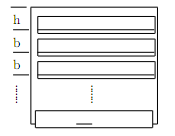
\includegraphics{./graphics/heightofpagebox.jpg}
\end{figure}
\end{comment}

\subsection{Dead cycles.} An execution of the OTR without shipping any material is called a \emph{dead cycle}. Dead cycles, have their uses and we will explain this a bit later on. However, long iterations that just return \textit{dead cycles} is an indication of an error somewhere. \tex counts the number of dead cycles in a counter named |\deadcycles| and stops the run if |\deadcycles >= \maxdeadcycles|.  In the \textit{plain} format |\maxdeadcycles| is set as 25 and in \latex as \the\deadcycles. |\maxdeadcycles = 100| is \the\maxdeadcycles. Each time |\shipout| is invoked, it resets |\deadcycles| to zero.

\begin{dispListing}
If the file is not included, reset \deadcycles, so that a long list of non-included
files does not generate an `Output loop' error.
115 \deadcycles\z@
116 \@nameuse{cp@#1}%
117 \fi
118 \let\@auxout\@mainaux}
\end{dispListing}


\subsection{\tex's Page Number.} The page number can come from any source. Salomon provides an example where the \textsc{OTR} typesets a page number from a |\count| variable. This is typeset centered below the printed area.

%\newpage
%
%Test
%\makeatletter
%
%\let\ltxxoutput\output
%\let\ltxlabel\label@name
%\output={{\let\label@name\@gobble
%  \shipout\vbox{
%  \box255\smallskip
%  \centerline{\thepage}}}
%}
%
%\vfill \penalty-10000
%
%\global\let\output\ltxxoutput
%\let\label@name\ltxlabel
%
%
%\makeatother


Notice that the output macro, just passes the contents of the box to |\shipout|. This is not actually a very good method, but is shown here to illustrate a point.

Note the |\tenrm| in the preceding example. It
is necessary because of the asynchronous nature of
the \otr. When the \otr is invoked, \tex can be
anywhere on the next page. Specifically, it could
be inside a group where a different font is used.
Without the |\tenrm|, that font (the current font)
would be used in the otr.
In the plain format, the |\count0| variable
serves as the page number, and the following two
macros are especially useful.




\subsection{The \texttt{\textbackslash vsplit} operation.} 

Supposed you have inserted the material required to go on a page on a big |\vbox|, but the material is a bit extra that what is required to fill a page exactly. You would need an operation to split the box in two. The |vsplit| operation does that. It is important to the understanding of OTR operations to have an intimate knowledge of |\vsplit|. Its syntax is: 

\begin{quote}
|\vsplit|\meta{box number} to \meta{dim}
\end{quote}

The result of the operation is a box. Most often it appears in an assignment such as: 

\begin{quote}
|\setbox1=\vsplit0 to2.6in| 
\end{quote}

This sets |\box1| to a
height of 2.6in, moves material from the top of
|\box0| to |\box1|, and keeps the remainder in |\box0|.

\begin{macro}{\loremlines}
It is important to remember that most of \tex's commands work with \latex as well. In Example~\ref{ex:loremlines}, we define a box to hold |lipsum| text in a two column layout. We want to define a macro that can split the box in as many lines as we require. 
\end{macro}

\begin{texexample}{Splitting a vbox}{ex:loremlines}
\newbox\one
\newbox\two
\long\gdef\loremlines#1#2{%
   \setbox\one=\vbox {#2}
   \setbox\two=\vsplit\one to #1\baselineskip
   \unvbox\two
   \gdef\boxone{#2}
}
\begin{multicols}{2}
\small
\loremlines{16}{\onepar}
\end{multicols}
\boxone

\setbox\one=\vbox{100}
\the\ht\one \\
\the\baselineskip
\the\splittopskip

\end{texexample}


\tex assumes that the new |\box1| may have to
be shipped out as part of the page. It therefore
places a glue similar to $h$ at the top of |\box1|.
This glue is called \docAuxCommand{splittopskip} and has a plain
format value of 10pt [348].

One important thing to note is that a box can only be split \textit{between} lines of text. 
If we split a box to another size, |\box1| will come out underfull.

Here is an \otr which splits the page, ships
out the top part and returns the rest to the MVL
(actually, to the recent contributions):

\begin{teXXX}
\output={\setbox0=\vsplit255 to1in
\shipout\box0 \unvbox255}
\end{teXXX}






\section{Communicating with the OTR: Marks}


The user can pass information to the output routine through \textit{marks}. Marks have the syntax

\begin{teX}
\mark{mark text}
\end{teX}

which is put in a mark item on the current vertical list. The mark text is subject to expansion
as in \cs{edef}.
If the mark is given in horizontal mode it migrates to the surrounding vertical lists like an
insertion item (see page Text By Topic 77); however, if this is not the external vertical list, the output routine
will not find the mark.

Marks are the main mechanism through which the output routine can obtain information
about the contents of the currently broken-off page, in particular its top and bottom. TEX sets
three variables:

{\obeylines
\cs{botmark} the last mark occurring on the current page;
\cs{firstmark} the first mark occurring on the current page;
\cs{topmark} the last mark of the previous page, that is, the value of \cs{botmark} on the previous
page.
}



If no marks have occurred yet, all three are empty; if no marks occured on the current page, all three variables are equal to the \cs{botmark} of the previous page. 

Marks can be used to get a section heading into the headline or footline of the page.

\begin{quote}
\begin{verbatim}
\def\section#1{ ... \mark{#1} ... }
\def\rightheadline{\hbox to \hsize
    {\headlinefont \botmark\hfil\pagenumber}}
\def\leftheadline{\hbox to \hsize
   {\headlinefont \pagenumber\hfil\firstmark}}
\end{verbatim}
\end{quote}

This places the title of the first section that starts on a left page in the left
headline, and the title of the last section that starts on the right page in
the right headline. Placing the headlines on the page is the job of the output
routine; see below.

It is important that no page breaks can occur in between the mark and the
box that places the title:

\emphasis{mark,nobreak}
\begin{teXXX}
\def\section#1{ ...
   \penalty\beforesectionpenalty
   \mark{#1}
   \hbox{ ... #1 ...}
   \nobreak
   \vskip\aftersectionskip
   \noindent}
\end{teXXX}

%%%%%%%%%%%% macro to put TeX references in right margin %%%%%%%% 
\newdimen\theight 
\def \TeXref#1{% 
             \vadjust{\setbox0=\hbox{\sevenrm\quad\quad\TeX book: #1}% 
             \theight=\ht0 
             \advance\theight by \dp0    \advance\theight by \lineskip 
             \kern -\theight \vbox to \theight{\rightline{\rlap{\box0}}% 
             \vss}% 
             }}% 
%%%%%%%%%%%%%%%%%%%%%%%%%%%%%%%%%%%%%%%%%%%%%%%%%%%%%%%%%%%%%%%%%%%%%%%%% 
 
However, useful these marks, sometimes an output routine (such as those found in \latexe needs to know why it was invoked. Knuth discusses in the \TeXref{396}  another method
that involves the value of the |\outputpenalty|. 
By testing for this value, it is possible to see what penalty occurred at a breakpoint;
any penalty of −10000, −10001, −10002, or less, forces the output routine to
act, hence different penalty values can be used to pass different messages. (When
the output routine puts material back on the list of contributions, it need not restore
the penalty at the breakpoint.) If output has been forced by a highly negative value
of |\outputpenalty|, the output routine can use |\vbox{\unvcopy255}| to discover how
full the page-so-far actually is. Underfull and overfull boxes are not reported when
|\box255| is packaged for use by the output routine, so there’s no harm in ejecting a
page prematurely if you want to pass a signal. (Set |\holdinginserts| positive to pass
a signal when the contents of |\box255| will be sent back through the page builder again,
if any insertions are present.)

Knuth also suggested another method that he called the \emph{dirtiest trick of all} that uses the depth 
of |\box255|. 

\section{Insertions}
Insertions are considered one of  the most  complex  topics in \tex. Many users master  topics  such 
as tokens,  file  I/O, macros,  and  even  OTRS  before they dare  tackle  insertions.  The  reason  is  that 
insertions  are  complex,  and  The \texbook, while 
covering all the relevant material, is somewhat cryptic regarding  insertions, and  lacks  simple examples. 
The  main  discussion  of  insertions takes  place  on 
[115-1251.  where \tex' s  registers  are also discussed. 
Examples  of  insertions are  shown, mostly  without 
explanations,  on  [363-364,  423-424].  A lot of what is described here is based on an article in TUGboat by David Salomon\footnote{\protect\url{http://www.tug.org/TUGboat/Articles/tb11-4/tb30salomon.pdf}}

Many users understand the idea of floats. Certain material to be typeset needs to be held in a buffer and inserted at different points on a page, for example a a figure that does not fit on a page it has to be inserted at the top of the next page. An \textit{insertion} is just a piece of a document that is generated at a certain point but appears at another point. Common examples are figures, footnotes and endnotes. Quoting Knuth:

\begin{quote}
  This  algorithm  is  admittedly  complicated, 
but  no  simpler  mechanism  seems  to  do  nearly 
as  much.
\end{quote}

\section{\protect\textbackslash shipout}

The primitive control sequence \docAuxCommand{shipout} is \tex's end game. It's syntax is quite simple:

\begin{quote}
|\shipout<box>|
\end{quote}

From TeXbook, Chapter 23: Output Routines, page 254:

\begin{quotation}
TeX’s primitive command |\shipout<box>| is what actually causes output. It sends the contents of the box to the dvi file, which is TeX’s main output file; after TeX has finished, the dvi file will contain a compact device-independent encoding of instructions that specify exactly what should be printed. When a box is shipped out, TeX displays the values of |\count0| through |\count9| on your terminal, as explained in Chapter 15; these ten counters are also recorded in the dvi file, where they can be used to identify the page. All of the |\openout, \closeout|, and |\write| commands that appear inside of the box are performed in their natural order as that box is being shipped out. Since a |\write| command expands macros, as explained in Chapter 21, TeX’s scanning mechanism might detect syntax errors while a |\shipout| is in progress. If  |\tracingoutput| is nonzero at the time of a \cs{shipout}, the contents of the box being shipped are written into your log file in symbolic form. You can say \cs{shipout} anywhere, not only in an output routine.
\end{quotation}


We can say:

\emphasize{shipout,vbox}
\begin{teXXX}
\shipout\vbox{%
  \hrule
  \medskip
  \lipsum[1-5]
  \medskip
  
  This is a Test for shipout
  
  \hrule
}
\end{teXXX}

\shipout\vbox{%
  \hrule
  \medskip
  \lipsum[1-5]
  \medskip
  \centering
  \textbf{Sample: }{This is a Test for shipout}
  \hrule
}

Since the output box handled by \tex still holds material the page is shown in the previous page. There is no page numbers or headers and it just shows he lorem-ipsum text and a primitive caption at the bottom. I have written the example to show the difference between the logical and actual pages. TeX does not care how the page will look, it will assemble it put headers, page numbers and pass it on to shipout. Shipout will then insert it to the dvi file, which will hold all teh instructions to print a real page.

We can modify the example to add our head and foot. 

\begin{texcode}{Shipout}{ex:ship2}
This will print by the normal routine

\long\gdef\boxit#1#2{\hbox{\vrule \vbox{\hrule\kern#2pt\hbox{%
\kern#2pt\vbox{#1}\kern#2pt}\kern#2pt\hrule}\vrule}}

\makeatletter
\shipout\vbox {%
  \vskip\topsep\relax
  \vskip\headsep
   \@thehead
   \vskip30pt
    \boxit{
      \lipsum[1-5]
      }{2}
   \vskip30pt
   \@thefoot   
}
\makeatother 
\end{texcode}

\latexe's output routine takes care of all the page geometry, the details to set up the headers and footers, but most importantly intercepts teh contents of the output box measure it, cuts it inserts the inserts such as footnotes and figures, margin notes, separates the text in two columns if necessary and so on. 

\long\gdef\boxit#1#2{\hbox{\vrule \vbox{\hrule\kern#2pt\hbox{%
\kern#2pt\vbox{#1}\kern#2pt}\kern#2pt\hrule}\vrule}}
\makeatletter
\shipout\vbox {%
  \vskip\topsep\relax
  \vskip\headsep
   \@thehead
   \vskip30pt
    \boxit{
      \lipsum[1-5]
      }{2}
   \vskip30pt
   \@thefoot   
}
\makeatother 



An output routine will prepare the virtual page and pass it onto a 

Here is an OTR for a \textit{framed} page. It surrounds the
page with double rules on all sides, and centers the
page number below the double box. Note that the
page shipped out is wider and taller than \cs{box255}.
The value of \cs{hsize} in this case is, therefore, not
the width of the final page shipped out, but the
width of the text lines in \cs{box255}.

Macro \cs{frameit} typesets text and surrounds it
with 4 rules (see [Ex. 21.3]). Parameter \#2 is the
space between the rules and the text. \#1 is a box
containing the text.

\emphasis{output,shipout}
\begin{texcode}{Example of simple output routine}{ex:output1}
\def\frameit#1#2{%
 \vbox{\hrule
  \hbox{%
    \vrule \kern#2pt
      \vbox{\kern#2pt #1
         \kern#2pt}%
      \kern#2pt\vrule}
\hrule}}

\output={
   \shipout\vbox{
   \boxit{\frameit{\box255}9}
      \medskip
      \centerline{Test Framed Page}}
  \advancepageno}
\end{texcode}

 

So far we did not care if the height of the page is right or not. In production code the shipout holds
a box, which has been produced by \tex. Any material we add to it, must not affect the dimensions of the box.
If we do and is too big the drivers will probably clip it.


Plain TeX has an output routine that takes care of  simple things like page numbering and insertions
using \cs{footnote} and \cs{topinsert}. 


So far we have examined the \tex OTR in detail. I hope it has given you enough understanding, not only to write your own output routine, but also to now be ready to study the \latex output routine, which is much more complicated. We have so far seen that  when \tex 
is typesetting pages of continuous text, it will gather material until it can find a least-cost page break intended to
make the gathered material fit the \cs{pagegoal} size. The
gathered material will then be placed into |\box255| and
the output routine stored in the token register \cs{output}
will be processed in a group of its own. 

Usually it will
arrange the gathered material in some way, add headers,
footlines and page numbers, and ship the gathered results out in typeset form with the \cs{shipout} command.
At the time of the \cs{shipout} command all \cs{open} and
\cs{write} commands stored in the box shipped out are expanded and written out. This is what makes it possible to have page labels corresponding to the actual page
numbers at the time of shipout: the corresponding info
is written to the |.aux| file at that time.
The output routine may decide to place material
back on the main vertical list instead of shipping it out. Its ob is to check if it can have a break, if it can it will ship the page out. If it cannot it will palce the material back on the main vertical list. 

\section{\LaTeX\  output routines}


\LaTeX\ output routine is described in \texttt{ltoutput.dtx}. You should also have a look at \texttt{ltfloat.dtx}. The algorithm is revisited i \latex3 and Frank Mittelbach, published a paper
\footnote{\protect\url{http://www.latex-project.org/papers/xo-pfloat.pdf}} in which he explains some of the problems facing the team, when dealing with the output routine.


Information on the output routine is rather scarce. Best source is a series of  articles in the TUGBoat by David Salomon.

\href{http://www.tug.org/TUGboat/Articles/tb11-1/tb27salomon.pdf}{Output Routines: Examples and Techniques. Part I: Introduction and Examples.}

\href{http://www.tug.org/TUGboat/Articles/tb11-2/tb28salomon.pdf}{Output Routines: Examples and Techniques. Part II: OTR Techniques}

\href{http://www.tug.org/TUGboat/Articles/tb11-4/tb30salomon.pdf}{Output Routines: Examples and Techniques. 
Part III: Insertions}

\href{http://www.tug.org/TUGboat/Articles/tb15-1/tb42salomon-output.pdf}{Output routines: Examples and techniques Part IV: Horizontal techniques}


David Kastrup's article \href{http://www.tug.org/TUGboat/Articles/tb24-3/kastrup.pdf}{Output Routine Requirements for Advanced Typesetting Tasks} (Proceedings of EuroTEX 2003) otlined some of the difficult areas and specifications for generic routines

The standard blocks are well described above and most tasks could be accomplished 
by rather working from
standard building blocks like \textit{insertion lists}, \textit{here points},
default mechanisms for \textit{margin notes} and so on.


%\section{Calling the output routine}
%
%The output routine is called either by TeX's normal page-breaking
%mechanism, or by a macro putting a penalty < or = -10000 in the output
%list. In the latter case, the penalty indicates why the output
%routine was called, using the following code.
%penalty reason
%
%\begin{longtable}{ll}
%\toprule
%penalty &reason\\
%\midrule
%-10000  &\ pagebreak\\
%~       &\ newpage\\
%-10001  &clearpage (\ penalty -10000 \ vbox{}| \ penalty -10001)|\\
%-10002  &float insertion, called from horizontal mode\\
%-10003 &float insertion, called from vertical mode.\\
%-10004 &float insertion.\\
%\bottomrule
%\end{longtable}
%\medskip
%
%Note: A |float| or |marginpar| puts the following sequence in the output
%list: 
%
%\begin{enumerate}
%\item a penalty of -10004,
%
%\item a null |\vbox|
%
%\item a penalty of -10002 or -10003.
%\end{enumerate}
%
%This solves two special problems:
%
%\begin{enumerate}
%\item If the float comes right after a |\newpage| or |\clearpage|,
%then the first penalty is ignored, but the second one
%invokes the output routine.
%
%\item If there is a split footnote on the page, the second 'page'
%puts out the rest of the footnote
%\end{enumerate}
%
%\latex first defines some helper routines and increase the \cs{maxdeadcycles}. The helper macros are for
%manipulating lisst.
%
%\begin{teX}
% \maxdeadcycles = 100
% \let\@elt\relax
% \def\@next#1#2#3#4{\ifx#2\@empty #4\else
%   \expandafter\@xnext #2\@@#1#2#3\fi}
%   \@next \CS \LIST {NONEMPTY}{EMPTY} == %% NOTE: ASSUME
%\@elt = \relax
% BEGIN assume that \LIST == \@elt \B1 ... \@elt \Bn
% if n = 0
% then EMPTY
% else 
%   \CS :=L \B1
%   \LIST :=G \@elt \B2 ... \@elt \Bn
%   NONEMPTY
% fi
%END
%\end{teX}
%
%
%\begin{teX}
%11 \def\@xnext \@elt #1#2\@@#3#4{\def#3{#1}\gdef#4{#2}}
%
%12 \def\@testfalse{\global\let\if@test\iffalse}
%13 \def\@testtrue {\global\let\if@test\iftrue}
%14 \@testfalse}
%   }
%
%15 \def\@bitor#1#2{\@testfalse {\let\@elt\@xbitor
%16   \@tempcnta #1\relax #2}}
%
%17 \def\@xbitor #1{\@tempcntb \count#1
%18    \ifnum \@tempcnta =\z@
%19    \else
%20      \divide\@tempcntb\@tempcnta
%21    \ifodd\@tempcntb \@testtrue\fi
%22   \fi}
%\end{teX}
%
%
%\subsection{Float boxes and lists.} 
%A \textit{float list} consisting of the 
%floats in boxes |\boxa ... \boxN| has
%the form:
%
%|\@elt \boxa ... \@elt \boxN|
%where |\boxI| is defined by
%
%|\newinsert\boxI|
%
%Normally, |\@elt| is |\let| to |\relax|. A test can be performed on the
%entire 
%oat list by locally |\def|'ing |\@elt| appropriately and
%executing the list.
%This is a lot more efficient than looping through the list.
%\LaTeX\ defines float boxes as |bx@A| to |bx@R| to make them available for 
%inserts. These will be used later to define the lists that hold these boxes. 
%
%\latex now defines the float boxes. Each one is defined as an \cmd{\newinsert.}
%
%\begin{teXXX}
%\newinsert\bx@A
%...
%\newinsert\bx@I
%\newinsert\bx@J
%\newinsert\bx@K
%\newinsert\bx@L
%\newinsert\bx@M
%\newinsert\bx@N
%\newinsert\bx@O
%\newinsert\bx@P
%\newinsert\bx@Q
%\newinsert\bx@R
%\end{teXXX}
%
%
%
%Once these boxes are defined they are inserted in the |@freelist|. At this point all the other lists are defined.
%
%\emphasis{@freelist,@toplist,@botlist,@midlist,@currlist}
%\begin{teXXX}
%41 \gdef\@freelist{\@elt\bx@A\@elt\bx@B\@elt\bx@C\@elt\bx@D
%         \@elt\bx@E
%42                 \@elt\bx@F\@elt\bx@G\@elt\bx@H\@elt\bx@I\@elt\bx@J
%43                 \@elt\bx@K\@elt\bx@L\@elt\bx@M\@elt\bx@N
%44                 \@elt\bx@O\@elt\bx@P\@elt\bx@Q\@elt\bx@R}
%\end{teXXX}
%
%\startlineat{45}
%All the lists are defined initially to be empty.
%\begin{teXXX}
%45 \gdef\@toplist{}
%46 \gdef\@botlist{}
%47 \gdef\@midlist{}
%48 \gdef\@currlist{}
%49 \gdef\@deferlist{}
%50 \gdef\@dbltoplist{}
%51 \gdef\@dbldeferlist{}
%\end{teXXX}
%
%
%The lists are similar to those defined in \texttt{plain}.
%
%\begin{description}
%\item[\cs{@freelist}] : List of empty boxes for placing new 
%floats.
%\item[\string\@toplist] : List of 
%floats to go at top of current column.
%\item[\string\@midlist] : List of 
%floats in middle of current column.
%\item[\string\@botlist] : List of 
%floats to go at bottom of current column.
%\item[\string\@deferlist] : List of 
%floats to go after current column.
%\item[\string\@dbltoplist] : List of double-col. 
%floats to go at top of current
%page.
%\item[\string\@dbldeferlist] : List of double-column 
%floats to go on subsequent
%pages.
%
%\end{description}
%
%\begin{multicols}{2}
%Check was prudent when defining the newinsert boxes in order to reserve space and memory. The package \docpkg{morefloats} can be used to add more floats to this list. This should have definitely been included here in a revision.
%
%\subsection{Defining Layout parameters} All the page layout parameters are defined next. 
%
%\begin{teXXX}
%52 \newdimen\topmargin
%53 \newdimen\oddsidemargin
%54 \newdimen\evensidemargin
%55 \let\@themargin=\oddsidemargin
%56 \newdimen\headheight
%57 \newdimen\headsep
%58 \newdimen\footskip
%59 \newdimen\textheight
%60 \newdimen\textwidth
%61 \newdimen\columnwidth
%62 \newdimen\columnsep
%63 \newdimen\columnseprule
%64 \newdimen\marginparwidth
%65 \newdimen\marginparsep
%66 \newdimen\marginparpush
%\end{teXXX}
%
%Remember  that TeX knows little about a page. The problem is that TEX has no idea how
%wide and tall the paper is. All it knows is the
%left and top offsets, and the dimensions of the
%printed area (|\hsize| and |\vsize|). All these dimensions need to be calculated and adjustments made within the \otr.
%
%A document normally  starts by specifying:
%
%\begin{teXXX}
%\newdimen\paperheight
%\newdimen\paperwidth
%\paperheight=..in \paperwidth=..in
%\end{teXXX}
%
%
%\end{multicols}
%
%
%\subsection*{The AtBeginDvi}
%A box register is used  to put stuff that must appear before anything else
%in the |.dvi| file.
%
%The stuff in the box should not add any typeset material to the page when it
%is unboxed.
%
%\emphasis{AtBeginDvi,@begindvibox}
%
%\begin{teXXX}
%67 \newbox\@begindvibox
%68 \def \AtBeginDvi #1{%
%69 \global \setbox \@begindvibox
%70 \vbox{\unvbox \@begindvibox #1}%
%71 }
%\end{teXXX}
%
%\begin{teXXX}
%72 \newdimen\@maxdepth
%73 \@maxdepth = \maxdepth
%\end{teXXX}
%
%
%Some new registers for paperheight and paperwidth are defined:
%
%\begin{teXXX}
%74 \newdimen\paperheight
%75 \newdimen\paperwidth
%76 \newif \if@insert
%These should definitely be global:
%77 \newif \if@fcolmade
%78 \newif \if@specialpage \@specialpagefalse
%These should be global but are not always set globally in other les.
%79 \newif \if@firstcolumn \@firstcolumntrue
%80 \newif \if@twocolumn \@twocolumnfalse
%Not sure about these: two questions. Should things which must apply to a whole
%doument be local or global (they probably should be `preamble only' commands)?
%Are these three such things?
%81 \newif \if@twoside \@twosidefalse
%82 \newif \if@reversemargin \@reversemarginfalse
%83 \newif \if@mparswitch \@mparswitchfalse
%This counter has been imported from `multicol'.
%84 \newcount \col@number
%85 \col@number \@ne
%\end{teXXX}
%
%and a lot of other internal registers
%
%\begin{teX}
%86 \newcount\@topnum
%87 \newdimen\@toproom
%88 \newcount\@dbltopnum
%89 \newdimen\@dbltoproom
%90 \newcount\@botnum
%91 \newdimen\@botroom
%92 \newcount\@colnum
%93 \newdimen\@textmin
%94 \newdimen\@fpmin
%95 \newdimen\@colht
%96 \newdimen\@colroom
%97 \newdimen\@pageht
%98 \newdimen\@pagedp
%99 \newdimen\@mparbottom \@mparbottom\z@
%100 \newcount\@currtype
%101 \newbox\@outputbox
%102 \newbox\@leftcolumn
%103 \newbox\@holdpg
%104 \def\@thehead{\@oddhead} % initialization
%105 \def\@thefoot{\@oddfoot}
%\end{teX}
%
%
%\subsection{\texttt{\textbackslash clearpage}}
%
%\begin{macro}{\clearpage}
%The clearpage macro is a bit complicated, as it needs to avoid a complete empty page after a |\twocolumn[..]|. This prevents the text from the argument
%vanishing into a  float box, never to be seen again. We hope that it does not
%produce wrong formatting in other cases.
%\end{macro}
%
%\begin{teXXX}
%106 \def\clearpage{%
%107   \ifvmode
%108   \ifnum \@dbltopnum =\m@ne
%109     \ifdim \pagetotal <\topskip
%110       \hbox{}%
%111     \fi
%112   \fi
%113  \fi
%114 \newpage
%115 \write\m@ne{}%
%116 \vbox{}%
%117 \penalty -\@Mi
%118 }
%\end{teXXX}
%
%\subsection{The \texttt{\textbackslash clearpagedoublepage} macro} 
%
%\begin{macro}{cleardoublepage}
%This checks for odd and even pages by using the
%page counter |c@page|.  It also provides switches of twoside printing. 
%
%\numberlineat{119}
%\begin{teXXX}
%\def\cleardoublepage{%
%   \clearpage
%   \if@twoside 
%     \ifodd\c@page
%     \else
%       \hbox{}
%       \newpage
%       \if@twocolumn\hbox{}\newpage
%       \fi
%     \fi
%  \fi}
%\end{teXXX}
%\end{macro}
%
%Note the |\newpage| is defined a bit further on. This is a fairly simple definition, since most of the code that follows only gets a bit complicated with the twocolumn option. It sets the dimensions and the booleans to those appropriate for the |onecolumn| option. An important note we back to \tex's |\hsize|. Both the linewidth as well as the columnwidth are set to this.
%
%\begin{teXXX}
%123 \def\onecolumn{%
%124   \clearpage
%125   \global\columnwidth\textwidth
%126   \global\hsize\columnwidth
%127   \global\linewidth\columnwidth
%128   \global\@twocolumnfalse
%129   \col@number \@ne
%130   \@floatplacement
%     }
%\end{teXXX}
%
%\subsection{\string newpage.} 
%
%The |\newpage| macro is programmed defensively. The two checks at the beginning ensure that an item label or run-in section title
%immediately before a |\newpage| get printed on the correct page, the one before
%the page break.
%All three tests are largely to make error processing more robust; that is why
%they all reset the 
%flags explicitly, even when it would appear that this would be
%done by a |\leavevmode|.
%
%\begin{teXXX}
%131 \def \newpage {%
%132  \if@noskipsec
%133    \ifx \@nodocument\relax
%134      \leavevmode
%135      \global \@noskipsecfalse
%136    \fi
%137 \fi
%138 \if@inlabel
%139   \leavevmode
%140   \global \@inlabelfalse
%141 \fi
%142 \if@nobreak \@nobreakfalse \everypar{}\fi
%143 \par
%144 \vfil
%145 \penalty -\@M}
%\end{teXXX}
%
%An empty cols is defined. There is a note here, that an invisible rule might have been a better idea.
%
%\begin{teXXX}
%146 \def \@emptycol {\vbox{}\penalty -\@M}
%\end{teXXX}
%
%\subsection{The \string twocolumn macro.} This is the longest definition so far. We will leave it for a while and then come back. There are several bug fixes to the two-column stuff here. Firstly, like the onecolumn the page parameters are set to the correct parameters.
%
%
%\begin{teXXX}
%147 \def \twocolumn {%
%148 \clearpage
%149 \global\columnwidth\textwidth
%150 \global\advance\columnwidth-\columnsep
%151 \global\divide\columnwidth\tw@
%152 \global\hsize\columnwidth
%153 \global\linewidth\columnwidth
%154 \global\@twocolumntrue
%155 \global\@firstcolumntrue
%156 \col@number \tw@
%\end{teXXX}
%
%
%
%\section{The output macro}
%
%The setting of the \cs{output} is quite short but it belies its complexity.
%After having checked verious parameters it redirects to |@specialoutput|. This is the heart of the routines. Notice that \latex just fills in the token list of \tex's |output| routine, it does not attempt to redefine it or save it. 
%Should some hooks be defined here, life might have been made easier, however, what one can do is to first save the \latex output routine and then redefine the output as one may wish. Return to it can happen after it. If you take this approach, you should be careful of packages that redefine output, such as |multicol| and |longtable|. An approach such as this is taken by \citeauthor{revtex} in the \pkgname{revtex} class.\footcite[][This is a document class of the American Physical Society. It enables submission to any of the APS journals. Its distribution point is \protect\url{http://publish.aps.org/revtex4/}]{revtex}
%
%\emphasis{ifnum,fi,else,ifdimen,@specialoutput}
%\begin{teX}
%204 \output {%
%205 \let \par \@@par
%206 \ifnum \outputpenalty<-\@M
%207    \@specialoutput
%208 \else
%209    \@makecol
%210    \@opcol
%211    \@startcolumn
%212    \@whilesw \if@fcolmade \fi
%213      {%
%218      \@opcol\@startcolumn}%
%219 \fi
%220 \ifnum \outputpenalty>-\@Miv
%221 \ifdim \@colroom<1.5\baselineskip
%222 \ifdim \@colroom<\textheight
%223 \@latex@warning@no@line {Text page \thepage\space
%224 contains only floats}%
%225 \@emptycol
%226 % \if@twocolumn
%227 % \if@firstcolumn
%228 % \else
%229 % \@emptycol
%230 % \fi
%231 % \fi
%232 \else
%  233 \global \vsize \@colroom
%234 \fi
%235 \else
%236   \global \vsize \@colroom
%237 \fi
%238 \else
%239   \global \vsize \maxdimen
%240 \fi
%241 }
%\end{teX}
%
%
%
%\begin{teXXX}
%244 \gdef\@specialoutput{%
%245   \ifnum \outputpenalty>-\@Mii
%246     \@doclearpage
%247   \else
%248     \ifnum \outputpenalty<-\@Miii
%249         \ifnum \outputpenalty<-\@MM \deadcycles \z@ \fi
%250                 \global \setbox\@holdpg \vbox {\unvbox\@cclv}%
%251         \else
%252         \global \setbox\@holdpg \vbox{%
%253                 \unvbox\@holdpg
%254                 \unvbox\@cclv
%We must now remove the box added by the 
%oat mechanism and the \topskip
%glue therefore added above it by TEX.
%255                \setbox\@tempboxa \lastbox
%256                \unskip
%257 }%
%These two are needed as separate dimensions only by \@addmarginpar; for other
%purposes we put the whole size into \@pageht (see below).
%258                \@pagedp \dp\@holdpg
%259                \@pageht \ht\@holdpg
%260                \unvbox \@holdpg
%
%261                \@next\@currbox\@currlist{%
%262                \ifnum \count\@currbox>\z@
%Putting the whole size into \@pageht (see above).
%263                  \advance \@pageht \@pagedp
%264                  \ifvoid\footins \else
%265                    \advance \@pageht \ht\footins
%266                    \advance \@pageht \skip\footins
%267                    \advance \@pageht \dp\footins
%268                \fi
%\end{teXXX}
%
%
%
%\subsection{The \string @doclearpage macro.} This is an emergency action. It dumps everything: footnotes first and then floats. 
%
%
%\section*{The Kludgeins}
%
%The kludgeins are simply inserts that fool \tex in enlarging a page by a small amount, normally used to allow one or two lines of text to go in the same page.
%
%The two kludgeins mentioned in the kernel are are \cs{enlargethisspace} and its star version.\footnote{The Oxford English Dictionary (2nd ed., 1989) kludge entry cites one source for this word's earliest recorded usage, definition, and etymology: Jackson W. Granholm's 1962 "How to Design a Kludge" article, which appeared in the American computer magazine Datamation
%kludge  Also kluge. [J. W. Granholm's jocular invention: see first quot.; cf. also bodge v., fudge v.]
%
%'An ill-assorted collection of poorly-matching parts, forming a distressing whole' (Granholm); esp. in Computing, a machine, system, or program that has been improvised or 'bodged' together; a hastily improvised and poorly thought-out solution to a fault or 'bug'.
%
%The word 'kludge' is...derived from the same root as the German Kluge..., originally meaning 'smart' or 'witty'.... 'Kludge' eventually came to mean 'not so smart' or 'pretty ridiculous'.}
%
%
%
%\begin{teXX}
%\gdef \enlargethispage{%
%1198 \@ifstar
%1199 {%
%1203   \@enlargepage{\hbox{\kern\p@}}}%
%1204 {%
%1208   \@enlargepage\@empty}%
%1209 }
%\end{teXX}
%
%Adds |<dim>| to the height of the current column only. On the printed page the
%bottom of this column is extended downwards by exactly |<dim>| without having
%any effect on the placement of the footer; this may result in an overprinting.
%\cs{enlargethispage}.
%
%Similar to |\enlargethispage| but it tries to squeeze the column to be printed
%in as small a space as possible, ie it uses any shrinkability in the column. If the
%column was not explicitly broken (e.g. with |\pagebreak|) this may result in an
%overfull box message but except for this it will come out as expected (if you know
%what to expect).
%The star form of this command is dedicated to Leslie Lamport, the other we
%need for ourselves (FMi, CAR).
%These commands may well have unwanted if used soon before a\ldots
%
% 




\section{Packages}

OTR routines are notoriously difficult to debug and define. Some of the available packages at CTAN
can make the programming job easier.

The \pkg{everypage} package by Sergio Callegari provides hooks into the \latex\ internal commands to
to do actions on every page or on the current page. Specifically, actions  are performed \emph{before} the page is shipped, so they can be used to put watermarks \emph{in the background} of a page, or to
set the page layout. 

The package provides two hooks:

\emphasis{AddEverypageHook,AddThisPageHook}
\begin{teXXX}
  \AddEverypageHook{Test}
  \AddThisPageHook
\end{teXXX}

The package reminds in some sense
\pkgname{bobhook} by Karsten Tinnefeld, but it differs in the way in
 which the hooks are implemented, as detailed in the following.
 In some sense it may also be related to the package
 \pkgname{everyshi} by Martin Schroeder, but again the implementation
 is different.

 
 This program adds two \LaTeX\ hooks that get run when document
 pages are finalized and output to the |.dvi| or |.pdf|
 file. Specifically, one hook gets executed on every page, while the
 other is executed for the current page. Hook actions are are performed
 \emph{before} the page is output on the medium, and this is
 important to be able to play with the page layout or to put things
 \emph{behind} the page contents (e.g., watermarks such as an image,
 framing, the ``DRAFT'' word, and the like).
 
 The package reminds in some sense \pkg{bobhook} by Karsten
 Tinnefeld, but it differs in the way in which the hooks are
 implemented:
 


 \begin{enumerate}
 \item there is no formatting inherent in the hooks. If one wants to
   put some watermark on a page, it is his own duty to put in the
   hook the code to place the watermark in the right position. Also
   note that the hooks code should \emph{eat up no space} in the
   page.  Again, if the hooks are meant to place some material on the
   page, it is the duty of the hook programmer to put code in the
   hooks to pretend that the material has zero width and zero height.
   The implementation is \emph{lighter} than the \Lpack{bobhook} one,
   and possibly more flexible, since one is not limited by any
   pre-coded formatting for the hooks. On the other hand it is
   possibly more difficult to use. Nonetheless, it is easy to think
   of other packages relying on \Lpack{everypage} to deliver more
   user-friendly and \emph{task specific} interfaces. Already there
   are a couple of them: the package \Lpack{flippdf} produces
   mirrored pages in a PDF document and \Lpack{draftwatermark}
   watermarks document pages.
 \item similarly to \Lpack{bobhook} and \Lpack{watermark}, the
   package relies on the manipolatoin of the internal \LaTeX\ macro
   |\@begindvi| to do the job. However, the redefinition of
   |\@begindvi| is here postponed as much as possible, striving to
   avoid interference with other packages using |\AtBeginDvi| or
   anyway manipulating |\@begindvi|. Specifically \Lpack{everypage}
   makes no special assumption on the initial code that |\@begindvi|
   might contain.
 \end{enumerate}



Also in some sense \pkgname{everypage} can be related to package
 \pkgname{everyshi} by Martin Schr\"oeder \cite{everyshi}, but it differs radically from
 it in the implementation. In fact,\pkgname{everypage} operates by
 manipulation of the |\@begindvi| macro, rather than at the
 lower level |\shipout| macro.

\section{hooking at shipout}

\begin{docCmd} {EveryShipout} {}
\begin{docCmd} {AtNextShipout} {}
This package provides the hooks \cs{EveryShipout} and 
  \cs{AtNextShipout} whose arguments are executed after the output 
  routine has constructed \cs{box255}, and before \cs{shipout} is 
  called.
\end{docCmd}
\end{docCmd}

An example application for this package would be a package for
 adding text to the bottom of each page.
 The  \pkgname{prelim2e} package adopts this method \citep{prelim2e}.\footcite{prelim2e}

The solution  uses is based on code developed in  |quire.tex| by
 Marcel R.~van der Goot.\footcite{quire}  

The \pkgname{prelim2e}  intercepts and modifies the |\box255|. 

\begin{teX}
44 \newcommand{\@Prelim@EveryShipout}{%
45 \bgroup
% First we save the dimensions of \box255: height, width and depth; and calculate
% the total height of \box255.
46 \dimen\z@=\wd\@cclv
47 \dimen\@ne=\ht\@cclv
48 \dimen\tw@=\dp\@cclv
49 \dimen\thr@@=\dimen1
50 \advance\dimen\thr@@ by \dimen\tw@
% Then we set \box255: A \vbox to the total height of \box255. In this a \hbox to
% the width of \box255 is included, in which \box255 is set.
51 \global\setbox\@cclv\vbox to \dimen\thr@@{%
52 \hb@xt@\dimen\z@{%
53 \box\@cclv%
54 \hss
55 }%
\end{teX}
To this we append the text produced by |\PrelimText|. It is put in a |\vbox to 0pt|
in which a |\hbox| to the width of |\box255| is included, in which |\PrelimText| is set.
We have to reset |\protect| because it is set to |\noexpand| by the output routine.

\begin{teXXX}
56 \vbox to \z@{%
57   \hb@xt@\dimen\z@{%
58     \let\protect\relax
59     \hfill\PrelimText\hfill
60   }%
61   \vss
62 }%
63   \vss
64 }%
\end{teXXX}

Finally we set the dimensions of |\box255| to the values they had before |\@Prelim@EveryShipout|.

\begin{teX}
65 \wd\@cclv=\dimen\z@
66 \ht\@cclv=\dimen\@ne
67 \dp\@cclv=\dimen\tw@
68 \egroup
69}
\end{teX}

Once the command is defined, it is hooked into the system via |\EveryShipout| when it is in draft mode. 

\begin{teX}
70 \if@prelim@draft
71 \EveryShipout{\@Prelim@EveryShipout}
72 \fi
\end{teX}

\section{How to place a background image}

One can use \tikzname to place a background image or some text on a page

First we define some utility macros:


\begin{teX}
\def\bg@contents{Draft}
\def\bg@color{red!45}
\def\bg@angle{60}
\def\bg@opacity{.5}
\def\bg@scale{15}
\def\bg@position{current page.center}
\def\bg@anchor{}
\def\bg@hshift{0}
\def\bg@vshift{0}
\end{teX}

A new command is then developed to describe the background material

\begin{teXXX}
\newcommand\bg@material{%
   \begin{tikzpicture}[remember picture,overlay]
   \node [rotate=\bg@angle,scale=\bg@scale,opacity=\bg@opacity,%
   xshift=\bg@hshift,yshift=\bg@vshift,color=\bg@color]
   at (\bg@position) [\bg@anchor] {\bg@contents};
  \end{tikzpicture}}%
\end{teXXX}


Once the background material has been defined we can place it on the page by simply calling:

\begin{teX}
\newcommand\BgThispage{\AddThispageHook{\bg@material}}
\end{teX}


The \pkgname{background}\footcite{background} package by \citeauthor has capitalized on two good packages the \tikzname and the \pkgname{everypage}.
\footcite{everypage} As most of modern
\tex programming works with |pdf| files, package developers prefer to use \tikzname methods for hooking directly into the pdf and thus avoid a trip into the output routine. If it is required then it hooks via the dvi or shipout commands.\footnote{These packages are loaded automatically by the \pkgname{phd-pkgmanager}.}



\vfill

\message{(total: \the\pagetotal
depth: \the\pagedepth
shrink: \the\pageshrink
stretch: \the\pagestretch}



 







































% 
%</driver>
% \fi
% 
%  \CheckSum{0}
%  \CharacterTable
%  {Upper-case    \A\B\C\D\E\F\G\H\I\J\K\L\M\N\O\P\Q\R\S\T\U\V\W\X\Y\Z
%   Lower-case    \a\b\c\d\e\f\g\h\i\j\k\l\m\n\o\p\q\r\s\t\u\v\w\x\y\z
%   Digits        \0\1\2\3\4\5\6\7\8\9
%   Exclamation   \!     Double quote  \"     Hash (number) \#
%   Dollar        \$     Percent       \%     Ampersand     \&
%   Acute accent  \'     Left paren    \(     Right paren   \)
%   Asterisk      \*     Plus          \+     Comma         \,
%   Minus         \-     Point         \.     Solidus       \/
%   Colon         \:     Semicolon     \;     Less than     \<
%   Equals        \=     Greater than  \>     Question mark \?
%   Commercial at \@     Left bracket  \[     Backslash     \\
%   Right bracket \]     Circumflex    \^     Underscore    \_
%   Grave accent  \`     Left brace    \{     Vertical bar  \|
%   Right brace   \}     Tilde         \~}
%
%
%
% \changes{1.0}{2018/01/26}{Converted to DTX file}
%
% \DoNotIndex{\newcommand,\newenvironment}
% \GetFileInfo{phd.dtx}
% 
%  \def\fileversion{v1.0}          
%  \def\filedate{2012/03/06}
% \title{The \textsf{phd} package.
% \thanks{This
%        file (\texttt{phd-utils.dtx}) has version number \fileversion, last revised
%        \filedate.}
% }
% \author{Dr. Yiannis Lazarides \\ \url{yannislaz@gmail.com}}
% \date{\filedate}
%
%
% 
% ^^A\maketitle
% 
% ^^A\frontmatter
%  ^^A\coverpage{./images/hine02.jpg}{Book Design }{Camel Press}
%  \newpage
% ^^A\secondpage
% \pagestyle{empty}
%
% \pagestyle{headings}
% \raggedbottom
% ^^A \StopEventually{}
%  \OnlyDescription
%
%  ^^A\StopEventually{\printindex}
%<*package>
% \CodelineNumbered
% \pagestyle{headings}
% 
% \chapter{Implementation}
%
% The implementation is divided into different parts. 
% These parts are sometimes placed smaller packages 
% to make their maintenance easier and also to enable,
% partial deployment.
% 	
% \begin{description}
%
%  \item[The Package Manager] This section is responsible 
%       for pre-loading  packages, resolving conflicts and 
%       providing all interfacing commands (see \docFile{phd-pkgmanager}).
%
%
%  \item[Scripts Manager] Manages the loading of scripts for the worlds 
%  laguages and scripts.
%
%  \item[Keys] Key values are managed through \pgfname. The package
%       \pkg{phd-handlers} provides some useful handlers, mostly used by
%       internally.
%
%  \item[Epigraphs] A small supplementary package for epigraphs.
%
%  \item[MWE] The package generates a large number
%		of Minimum Working Examples that we use for testing. 
%		Most of them can also used as examples for training 
%		or self-study.
%
%  \item[Counters] The package counters, is an extension to the current
%    \latexe package offering more functionality and close integration
%    with the rest of the |phd| packages.
%
% \end{description}
%
% \section{Preliminaries}
%
%   Standard file identification. We first announce the package 
%	 and require that it be used with \LaTeX2e. RE
%
%    \begin{macrocode}
\NeedsTeXFormat{LaTeX2e}[2017/04/15]%
\ProvidesPackage{phd-utils}[2018/1/13 v1.0 various useful utilities (YL)]%
\RequirePackage{expl3,xparse}
%    \end{macrocode}
%
% \section{spacing}
% {hspace} This is a \textit{hairspace}, here defined 
% as 1pt.
% {hquad} This is a half squad space
%
% \begin{docCommand}{hairspace}{}
%  Provides a space of 1pt
% \end{docCommand}
%    \begin{macrocode}
\ProvideDocumentCommand{\hairsp}{}{\hspace{1pt}}
%    \end{macrocode}
%    \begin{macrocode}
\ProvideDocumentCommand{\hquad}{}{\hskip0.5em\relax}% half quad space
% Sometimes, we need a little more horizontal spacing, too (used for symbols).
\ProvideDocumentCommand{\qqquad}{}{\qquad\quad}
\ProvideDocumentCommand{\ie}{}{\textit{i.\hairsp{}e}\xspace} %removed\@
\ProvideDocumentCommand{\eg}{}{\textit{e.\hairsp{}g.}\xspace}

\ProvideDocumentCommand{\BC}{ m }{\textsc{#1~bc}} %European Union Style Guide FIX

\ProvideDocumentCommand{\AD}{ m }{\textsc{ad~#1}} %European Union Style Guide FIX
\ProvideDocumentCommand{\bce}{ m }{\textsc{bce~#1}}
%    \end{macrocode}
% 
%
% \subsection{Standard phantom widths}
%
%    \begin{macrocode}
\newcommand\Zi{\phantom{0}} %Z conflicts with symbols 
\newcommand\ZZ{\phantom{00}}
\newcommand\ZZZ{\phantom{000}}
\newcommand\ZZZZ{\phantom{0000}}
\providecommand\newthought[1]{%
   \addvspace{1.0\baselineskip plus 0.5ex minus 0.2ex}%
   \noindent\textsc{#1}%
}
  \let\equation\gather             %% See tabu and hyperref docs
  \let\endequation\endgather
%    \end{macrocode}
% Support for quick setting of variables
%    \begin{macrocode}
\def\phddefvar#1#2{%
  \expandafter\def\csname PHDvar@#1\endcsname{#2}%
}
\def\phdifvar#1{%
  \expandafter\ifx\csname PHDvar@#1\endcsname\relax
    \expandafter\@secondoftwo
  \else
    \expandafter\@firstoftwo
  \fi
}
\def\phdusevar#1{%
  \phdifvar{#1}{%
    \csname PHDvar@#1\endcsname
  }{%
    variable #1\undefined
  }%
}
%    \end{macrocode}
% \section{Rules}
% We need to define a number of rules to use in typesetting styles.
%	We will use later on different styles of rules to decorate chapter headings.
%	We define a few here to simplify code later on.
%
%    \begin{macrocode}
\DeclareRobustCommand\thickrule{%
    \leavevmode \leaders \hrule height 2pt \hfill \kern \z@}
\DeclareRobustCommand\thinrule{\vrule width\textwidth height0.4pt depth0pt\relax}%
%
\DeclareRobustCommand\mediumrule{\rule{\textwidth}{0.8pt}}
%    Adjusted to get toc parameters in
\DeclareRobustCommand\Ruler{{\color{\tocchapternumberfill@cx}\rule[-4.1pt]{13cm}{0.4pt}}}
\DeclareRobustCommand\bottomline{\medskip
   \noindent\rule{\linewidth}{0.4pt}\medskip}
\DeclareRobustCommand\topline{\par\medskip
   \noindent\rule{\linewidth}{0.4pt}\medskip} 
%    \end{macrocode}
% 
% 
% 
%
%  Some chapter and sectioning heads include rules, we define them here for convenience.
%
%    \begin{macrocode}
\cxset{chapter rule color/.store in={\chapter@rule@color}}%
\cxset{chapter rule color=spot!30}
\DeclareRobustCommand\tikzrule{%
  \tikz [color=\chapter@rule@color, very thick, inner sep=0pt, outer sep=0pt]%
        \draw(0,0)--(\the\linewidth,0);
}%
%  The trim left is required to align the rule exactly
%    \begin{macrocode}           
%#1  options #2 width  #3 height           
\newcommand\drawrule[3][]{%
    \offinterlineskip
          \tikz [ name=s,trim left,
                   anchor=base,
                   draw=black, 
                 % double distance=.2pt,
                  line width=#3,
                  %very thick,
                  inner sep=0pt, 
                  outer sep=0pt,#1]   \draw(0,0)--(#2,0);
}
 \def\drawdoublerule#1#2{%
    \drawrule{#1}{#2}%
    \vskip2.5pt
    \drawrule{#1}{#2}%
 }
%    \end{macrocode}
%
% \section{Assertions}
%  These are used for testing modules, as well as for the self-running examples in tutorials.
%    \begin{macrocode}
%<@@=assert>
%    \end{macrocode}
% \begin{macro}{\TRUE,\FALSE,\PASS,\FAIL,\PASSED}
% Typesets the results of an assertion. 
%    \begin{macrocode}
\ExplSyntaxOn
\cs_set:Npn \l_@@_typeset_true: 
  {
    \meta{true code}
  }
\cs_set_nopar:Npn \TRUE { \l_@@_typeset_true: }
\cs_set_nopar:Npn \FALSE { \meta{false code} }
\cs_set_nopar:Npn \PASS { \tex_par:D \leavevmode {\sffamily\bfseries\textcolor{green!50!blue}{PASS}}\ ~}
\cs_set_nopar:Npn \FAIL { \tex_par:D \leavevmode {\sffamily\bfseries\textcolor{red!70!black}{FAIL}}\ ~}
%
\ProvideDocumentCommand{\PASSED}{ }{\textcolor{green!50!blue}{PASS}}

\cs_set:Npn \assert_eq_meaning:NN #1 #2 
  {
   \if_meaning:w #1#2 
     \PASS
     \else:
     \FAIL
   \fi:
  }

  
\cs_set:Npn \assert_not_eq_meaning:NN #1 #2 
  {
   \if_meaning:w #1#2 
     \FAIL
     \else:
     \PASS
   \fi:
  }  
\ExplSyntaxOff 
%    \end{macrocode}
% \end{macro}
%
%    \begin{macrocode}
%<@@=>
%    \end{macrocode}
%
%
% \ExplSyntaxOn
% \assert_eq_meaning:NN \macro\macro
% \assert_not_eq_meaning:NN \macro\macro
% \ExplSyntaxOff
%\iffalse
%</package>
%\fi
%
%
% \printindex
% \Finale
\endinput

%%% Good theorem styles
%%% github
http://web.evanchen.cc/exams/USAMO-2018-notes.pdf
https://github.com/vEnhance/dotfiles/blob/master/texmf/tex/latex/evan/evan.sty

